\def\year{2022}\relax
%File: formatting-instructions-latex-2022.tex
%release 2022.1
\documentclass[letterpaper]{article} % DO NOT CHANGE THIS
\usepackage{aaai22}  % DO NOT CHANGE THIS
\usepackage{times}  % DO NOT CHANGE THIS
\usepackage{helvet}  % DO NOT CHANGE THIS
\usepackage{courier}  % DO NOT CHANGE THIS
\usepackage[hyphens]{url}  % DO NOT CHANGE THIS
\usepackage{graphicx} % DO NOT CHANGE THIS
\urlstyle{rm} % DO NOT CHANGE THIS
\def\UrlFont{\rm}  % DO NOT CHANGE THIS
\usepackage{natbib}  % DO NOT CHANGE THIS AND DO NOT ADD ANY OPTIONS TO IT
\usepackage{caption} % DO NOT CHANGE THIS AND DO NOT ADD ANY OPTIONS TO IT
\DeclareCaptionStyle{ruled}{labelfont=normalfont,labelsep=colon,strut=off} % DO NOT CHANGE THIS
\frenchspacing  % DO NOT CHANGE THIS
\setlength{\pdfpagewidth}{8.5in}  % DO NOT CHANGE THIS
\setlength{\pdfpageheight}{11in}  % DO NOT CHANGE THIS
%
% These are recommended to typeset algorithms but not required. See the subsubsection on algorithms. Remove them if you don't have algorithms in your paper.
\usepackage{algorithm}
% \usepackage{algorithmic}
% \usepackage[ruled,linesnumbered]{algorithm2e}
%\usepackage{algpseudocode}

% Wenzhen Added
\usepackage{booktabs}
\usepackage{multirow}

% These are are recommended to typeset listings but not required. See the subsubsection on listing. Remove this block if you don't have listings in your paper.
\usepackage{newfloat}
\usepackage{subfig}
\usepackage{listings}
\lstset{%
	basicstyle={\footnotesize\ttfamily},% footnotesize acceptable for monospace
	numbers=left,numberstyle=\footnotesize,xleftmargin=2em,% show line numbers, remove this entire line if you don't want the numbers.
	aboveskip=0pt,belowskip=0pt,%
	showstringspaces=false,tabsize=2,breaklines=true}
\floatstyle{ruled}
\newfloat{listing}{tb}{lst}{}
\floatname{listing}{Listing}

%
%\nocopyright
%
% PDF Info Is REQUIRED.
% For /Title, write your title in Mixed Case.
% Don't use accents or commands. Retain the parentheses.
% For /Author, add all authors within the parentheses,
% separated by commas. No accents, special characters
% or commands are allowed.
% Keep the /TemplateVersion tag as is
\pdfinfo{
/Title (AAAI Press Formatting Instructions for Authors Using LaTeX -- A Guide)
/Author (AAAI Press Staff, Pater Patel Schneider, Sunil Issar, J. Scott Penberthy, George Ferguson, Hans Guesgen, Francisco Cruz, Marc Pujol-Gonzalez)
/TemplateVersion (2022.1)
}

% DISALLOWED PACKAGES
% \usepackage{authblk} -- This package is specifically forbidden
% \usepackage{balance} -- This package is specifically forbidden
% \usepackage{color (if used in text)
% \usepackage{CJK} -- This package is specifically forbidden
% \usepackage{float} -- This package is specifically forbidden
% \usepackage{flushend} -- This package is specifically forbidden
% \usepackage{fontenc} -- This package is specifically forbidden
% \usepackage{fullpage} -- This package is specifically forbidden
% \usepackage{geometry} -- This package is specifically forbidden
% \usepackage{grffile} -- This package is specifically forbidden
% \usepackage{hyperref} -- This package is specifically forbidden
% \usepackage{navigator} -- This package is specifically forbidden
% (or any other package that embeds links such as navigator or hyperref)
% \indentfirst} -- This package is specifically forbidden
% \layout} -- This package is specifically forbidden
% \multicol} -- This package is specifically forbidden
% \nameref} -- This package is specifically forbidden
% \usepackage{savetrees} -- This package is specifically forbidden
% \usepackage{setspace} -- This package is specifically forbidden
% \usepackage{stfloats} -- This package is specifically forbidden
% \usepackage{tabu} -- This package is specifically forbidden
% \usepackage{titlesec} -- This package is specifically forbidden
% \usepackage{tocbibind} -- This package is specifically forbidden
% \usepackage{ulem} -- This package is specifically forbidden
% \usepackage{wrapfig} -- This package is specifically forbidden
% DISALLOWED COMMANDS
% \nocopyright -- Your paper will not be published if you use this command
% \addtolength -- This command may not be used
% \balance -- This command may not be used
% \baselinestretch -- Your paper will not be published if you use this command
% \clearpage -- No page breaks of any kind may be used for the final version of your paper
% \columnsep -- This command may not be used
% \newpage -- No page breaks of any kind may be used for the final version of your paper
% \pagebreak -- No page breaks of any kind may be used for the final version of your paperr
% \pagestyle -- This command may not be used
% \tiny -- This is not an acceptable font size.
% \vspace{- -- No negative value may be used in proximity of a caption, figure, table, section, subsection, subsubsection, or reference
% \vskip{- -- No negative value may be used to alter spacing above or below a caption, figure, table, section, subsection, subsubsection, or reference

\setcounter{secnumdepth}{0} %May be changed to 1 or 2 if section numbers are desired.

% The file aaai22.sty is the style file for AAAI Press
% proceedings, working notes, and technical reports.
%

% Title

% Your title must be in mixed case, not sentence case.
% That means all verbs (including short verbs like be, is, using,and go),
% nouns, adverbs, adjectives should be capitalized, including both words in hyphenated terms, while
% articles, conjunctions, and prepositions are lower case unless they
% directly follow a colon or long dash
% \title{DocBed: End-to-End OCR Solution for Documents with Complex Layouts}
% \author{Paper ID: 11030}
%\affiliations{Keywords: }
% \author{
%     %Authors
%     % All authors must be in the same font size and format.
%     Written by AAAI Press Staff\textsuperscript{\rm 1}\thanks{With help from the AAAI Publications Committee.}\\
%     AAAI Style Contributions by Pater Patel Schneider,
%     Sunil Issar,\\
%     J. Scott Penberthy,
%     George Ferguson,
%     Hans Guesgen,
%     Francisco Cruz\equalcontrib,
%     Marc Pujol-Gonzalez\equalcontrib
% }
% \affiliations{
%     %Afiliations
%     \textsuperscript{\rm 1}Association for the Advancement of Artificial Intelligence\\
%     % If you have multiple authors and multiple affiliations
%     % use superscripts in text and roman font to identify them.
%     % For example,

%     % Sunil Issar, \textsuperscript{\rm 2}
%     % J. Scott Penberthy, \textsuperscript{\rm 3}
%     % George Ferguson,\textsuperscript{\rm 4}
%     % Hans Guesgen, \textsuperscript{\rm 5}.
%     % Note that the comma should be placed BEFORE the superscript for optimum readability
%     2275 East Bayshore Road, Suite 160\\
%     Palo Alto, California 94303\\
%     % email address must be in roman text type, not monospace or sans serif
%     publications22@aaai.org
% %
% See more examples next
%}

%Example, Single Author, ->> remove \iffalse,\fi and place them surrounding AAAI title to use it
\iffalse
\title{My Publication Title --- Single Author}
\author {
    Author Name
}
\affiliations{
    Affiliation\\
    Affiliation Line 2\\
    name@example.com
}
\fi

% \iffalse
%Example, Multiple Authors, ->> remove \iffalse,\fi and place them surrounding AAAI title to use it
\title{\title{DocBed: A Multi-Stage OCR Solution for Documents with Complex Layouts}}
\author {
    % Authors
    Wenzhen Zhu,\textsuperscript{\rm 1}
    Negin Sokhandan, \textsuperscript{\rm 1}
    Guang Yang, \textsuperscript{\rm 1}
    Sujitha Martin, \textsuperscript{\rm 1}
    Suchitra Sathyanarayana \textsuperscript{\rm 1}
}
\affiliations {
    % Affiliations
    \textsuperscript{\rm 1} Amazon Machine Learning Solutions Lab \\
    \{wenzhu, ngnsl, yaguan, sujimart, suchisat\}@amazon.com
}
%\fi


% REMOVE THIS: bibentry
% This is only needed to show inline citations in the guidelines document. You should not need it and can safely delete it.
\usepackage{bibentry}
% END REMOVE bibentry

\begin{document}

\maketitle

\begin{abstract}
Digitization of newspapers is of interest for many reasons including preservation of history, accessibility and search ability, etc. While digitization of documents such as scientific articles and magazines is prevalent in literature, one of the main challenges for digitization of newspaper lies in its complex layout (e.g. articles spanning multiple columns, text interrupted by images) analysis, which is necessary to preserve human read-order. This work provides a major breakthrough in the digitization of newspapers on three fronts: first, releasing a dataset of 3000 fully-annotated, real-world newspaper images from 21 different U.S. states representing an extensive variety of complex layouts for document layout analysis; second, proposing layout segmentation as a precursor to existing optical character recognition (OCR) engines, where multiple state-of-the-art image segmentation models and several post-processing methods are explored for document layout segmentation; third, providing a thorough and structured evaluation protocol for isolated layout segmentation and end-to-end OCR.

\end{abstract}

%%%%%%%%% BODY TEXT
\section{Introduction}
In the digital age, information that used to be spread by printouts is disseminated at unforeseen speeds through digital formats. In parallel to the inventions of new types of media, an increasing number of archives and libraries are trying to create digital repositories with new technologies \cite{DBLP:journals/firstmonday/Cox07}. Digitization allows for preservation by creating an accessible surrogate, while at the same time enabling easier storage, indexing, and faster search.

%In this work, we present a fully-annotated high-quality real-world document dataset with an extensive variety of complex layouts. 

The objective of this work is to build and investigate systems that can generalize well to the digitization of historical newspapers, where digitization here refers to extracting content (e.g. text, image, ads) in human read-order.
%preserving human read-order and ability to discern one type of content from another.
This is challenging because there are many variations among old newspapers, including font sizes and styles, number of columns, column width, column separators, advertisement placement, image placements, table style, break in continuity of articles across multiple columns, text versus non-text ratio, etc., to name a few. To address these challenges, this paper makes three contributions:
\begin{itemize}
    \item a new dataset of 3000 scanned pages sampled from 21 different newspaper publications spread across the U.S. states over a few decades and annotated with bounding boxes for seven categories.
    \item an end-to-end framework for document layout analysis that uses a variety of advanced segmentation and detection techniques, such as Mask R-CNN from Detectron2 \cite{wu2019detectron2} and Segmentation Transformer \cite{Zheng_2021_CVPR}, and several post-processing algorithms (that optimize the number of API calls and improve text recognition metrics) to handle various context-aware text extraction tasks, as a precursor to existing OCR engines like Amazon Textract and Tesseract.
    \item two benchmarking pipelines that allow evaluation of isolated layout segmentation and end-to-end text recognition.
\end{itemize}

%First, %to capture these variations% in a dataset for training and testing purposes,
%to capture the challenging variations of newspaper layouts, we introduce and release a new dataset sampled from 21 different newspaper publications spread across the U.S. states over a few decades. 
%More specifically, the dataset encompasses newspapers from more 21 different U.S. states and primarily spans from the 1880s up to the 1920s. 

%In addition to the above, we develop an end-to-end framework for document layout analysis that uses a variety of advanced segmentation and detection techniques such as Detectron2 \cite{wu2019detectron2} and Segmentation Transformer \cite{Zheng_2021_CVPR} along with the Amazon Textract OCR engine and several post-processing algorithms (that optimize the number of API calls and improve text recognition metrics) to handle various context-aware text extraction tasks. The proposed framework is packaged with two benchmarking pipelines that allow evaluation of isolated layout segmentation and end-to-end text recognition. %of layout segmentation and text recognition modules separately.

% The flexible and modular structure of the proposed pipeline turns it into a general and handy tool for different document analysis applications. 
% For example, different OCR engines, segmentation models or post-processing algorithms can be separately plugged into the pipeline for analysis purposes.
 
%\subsection{Challenges}

%\paragraph{OCR Engine Limitations} Common OCR engines often fail when a given document has a fairly complex layout or a scanned image file size is too large.

\section{Related Work}
Document layout analysis is a critical step in document digitization and is often split into two tasks: page segmentation and region classification. The objective is to infer the underlying structure of an unstructured digital document and parse it into structured formats so that each article can be properly indexed. Previous work on this topic can be mainly grouped into two categories: (1) layout analysis methods and (2) data collection and layout label generation aiming to include larger varieties of document types. 
% ;and (3) evaluation framework creation and methods benchmark.    

% \subsection{Methods for Layout Analysis}
Various rule-based algorithms have been proposed for document layout analysis. These methods can be divided into bottom-up and top-down approaches. Bottom-up approaches first classify small components of an image and then cluster similar components to form regions. On the other hand, top-down approaches cut the image recursively in vertical and horizontal directions along white spaces or boundary lines. \cite{DBLP:conf/icdar/Smith09} used a bottom-up method to first generate initial data-type hypothesis and then applied a top-down method to impose structural regions, which later became the layout analysis component of the Tesseract engine. \cite{DBLP:journals/jodl/KlampflGJK14} applied a bottom-up approach to first extracts text blocks and then formed geometrical relations via graph-based approaches between these blocks. 

However, as these methods are highly dependent on heuristics and strategic thresholds, they are often greedy and sub-optimal. To increase the flexibility of the segmentation methods to dynamically adapt the local thresholds to local variations, some globally optimized methods were proposed. \cite{DBLP:conf/icdar/AgrawalD09a}
proposed a global page segmentation method based on Voronoi and Docstrum features.
% proposed a segmentation method based on Voronoi and Docstrum features which globally adapts to page content to determine algorithm parameters.
\cite{DBLP:conf/icvgip/DasigiJJ08} formulated the document segmentation into an optimal spectral partitioning problem, for which a closed form solution can be achieved instead of classic adhoc solutions.

Lately, the applicability of deep neural networks methods has gained a lot of attention. Fully convolutional networks (FCN) has been explored in multiple studies \cite{DBLP:conf/icfhr/OliveiraSK18} \cite{DBLP:conf/das/WickP18} \cite{DBLP:conf/icdar/MeierSSAC17}. Later, proposals were made to include textual features to achieve better and finer page segmentation and region classification \cite{DBLP:journals/corr/abs-2002-06144} \cite{DBLP:conf/emnlp/KattiRGBBHF18}. 

% \subsection{Dataset and Annotations Creation} 
% It is observed that each document segmentation method discussed above tends to focus on specific type of document. However, the variety of documents that need digitization in real life is large. In addition, the size of publicly available datasets for document layout analysis is quite small compared to established datasets for other computer vision research topics. There have been a few studies trying to address this issue.
A series of efforts have been made in the ICDAR challenges, led by researchers in the Pattern Recognition and Image Analysis (PRImA) Research Lab, to increase the diversity of document types for layout analysis. \cite{DBLP:conf/icdar/AntonacopoulosBPP09} created a dataset with a wide selection of complex and contemporary documents. The dataset consisted of 1240 images with corresponding accurate ground-truth and extensive metadata. However, particular emphasis was placed on magazines and technical journals. Old documents pose unique challenges compared to the contemporary documents due to lower print qualities and more complex layouts. To accommodate the need for digitizing historical document archives, \cite{DBLP:conf/icdar/ClausnerPPA15} presented a dataset comprising over 500 images of newspapers mostly published around World War I period.
% as they contained numerous important historical events. 
\cite{DBLP:conf/icpr/LieblB20} annotated 104 BBZ newspaper images by manually applying drawings
% onto a layer with a smart blending setting 
in a standard photo editing application. To get around the dataset size limit due to manual annotations requirements, \cite{DBLP:conf/icdar/ZhongTJ19} developed PubLayNet dataset by automatically matching XML representations with over 1 million article pdfs publicly available on PubMed Central. However, this method only applies to contemporary documents with XML representations.
% required for web display. 
% \subsection{Methods Evaluation} 
% \cite{DBLP:conf/icpr/LieblB20} performed a systematic evaluation on 11 different deep neural network segmentation methods based on the pixel level evaluation. Besides the commonly used pixel accuracy, F1 score and intersection over union (IoU), a new Matthews Correlation Coefficient (MCC) were used. In addition, they measured the influence of the number of labels and the number of training pages on the segmentation quality using MCC.

% In the series of ICDAR Page Segmentation competitions since 2001, objective evaluation framework and schema have been discussed. \cite{DBLP:conf/icdar/ClausnerAP17} described in detail how they evaluated different document analysis methods. For layout analysis evaluation, several situations (i.e. merger, split, miss, false detection and misclassification) were defined based on the identified correspondences between ground truth and predicted segments and each situation was quantified by an error rate. For text recognition evaluation, character-based and word-based measures were proposed. \cite{DBLP:journals/prl/ClausnerPA20} proposed a flexible character accuracy measure (Flex Character Accuracy) to handle the influence of determined read order. A Bag-of-Words measure was used to count how many words have been correctly recognized which disregarded read order entirely.     

\section{Datasets}
Two data sources are used in this work. The first is proposed as a part of our contributions and is primarily used for page layout segmentation analysis and benchmarking. The second is an existing dataset, which is used for benchmarking the benefits of page layout segmentation on OCR results.

%In order to investigate the performance of the proposed methods and demonstrate its generality, EulerEye is applied on two tasks related to document digitization. Document layout segmentation are evaluated on COCO-like evaluator for both with class and without class. Additional dataset is used to show the OCR final metrics. (this needs to be rewrite)
%\subsection{Layout Segmentation}

\paragraph{NewsNet7: Newspaper Layout Segmentation Dataset}
For layout segmentation analysis and benchmarking, 3000 images are sampled from an online database hosted at Chronicling America and produced by the National Digital Newspaper Program (NDNP), and annotated for page layout segments to create a new dataset called NewsNet7. Chronicling America is a website containing a large database of historic newspapers spanning all 50 states of the U.S. and over almost two centuries, from the late 1700s to the mid 1900s. In order to capture a wide variety of complex layouts, NewsNet7 is sampled from different newspaper publishers spread across 21 different U.S. states. To maintain a certain degree of consistency across the samples, each sample was required to be of a certain resolution (i.e. at least 4 megabytes). In addition, the samples were randomly sampled such that it covered more uniformly within the time span of its respective publisher and represented different pages of an issue. 

The extracted 3000 samples of newspaper images were manually annotated for page layout segmentation, in the form of bounding boxes for each of the following categories:
\begin{itemize}
    \item \textbf{Header}: Newspaper title related headers, usually appears at the very top.
    \item \textbf{Article title}: The title of each individual article which is followed by article body. 
    % The difference between title and body of text is that at least the first letter of each word in the "title" is capital.
    \item \textbf{Article body}: A body of text which follows an article title. Article body may span multiple columns and if so, annotations are broken into multiple bounding boxes, where each bounding box is restricted to span only one column.
    \item \textbf{Advertisement}: Text sections with visually more artistic and irregular formatting (e.g. different font style and size). To discern between ad and article, only visual cues were used and no consideration was given to content.
    \item \textbf{Image}: Represents art, photo, illustrations, etc.
    % Image may span anywhere from less than full width of a column to multiple columns. If an image is within an article or ad, in addition to labelling the entirety of the article or ad, image is explicitly labelled within as well. 
    \item \textbf{Table}: Arrangement of data in rows and columns (normally comes in key-value pairs). 
    % If a table is within an article or ad, in addition to labelling the entire article or ad, table is explicitly labelled within as well.
    \item \textbf{Other}: Is assigned to segments not falling into any of the above categories.
\end{itemize}

An illustration of page layout segmentation annotation is shown in Figure \ref{fig:NewspaperNet15}.
% with multiple instances of a subset of categories. 
Table 1 summarizes the number of instance each category appears in the NewsNet7 dataset and how the dataset is split into train and test.

% \ref{table:NewsNet7_data_stats}
%Chronicling America is a Website providing access to information about historic newspapers and select digitized newspaper pages, and is produced by the National Digital Newspaper Program (NDNP). NDNP, a partnership between the National Endowment for the Humanities (NEH) and the Library of Congress (LC), is a long-term effort to develop an Internet-based, searchable database of U.S. newspapers with descriptive information and select digitization of historic pages. Supported by NEH, this rich digital resource will be developed and permanently maintained at the Library of Congress. An NEH award program will fund the contribution of content from, eventually, all U.S. states and territories." From `https://chroniclingamerica.loc.gov/about/`, need to rephrase and abbreviate.

%\paragraph{Our Dataset}

%Since the available public datasets suffers from quantity and image quality, we Amazon Machine Learning Solutions Lab decided to make our own dataset. We selected 3000 newspapers from Chronicling America from 21 different publishers.
    
 \begin{figure}[h]
  \centering
  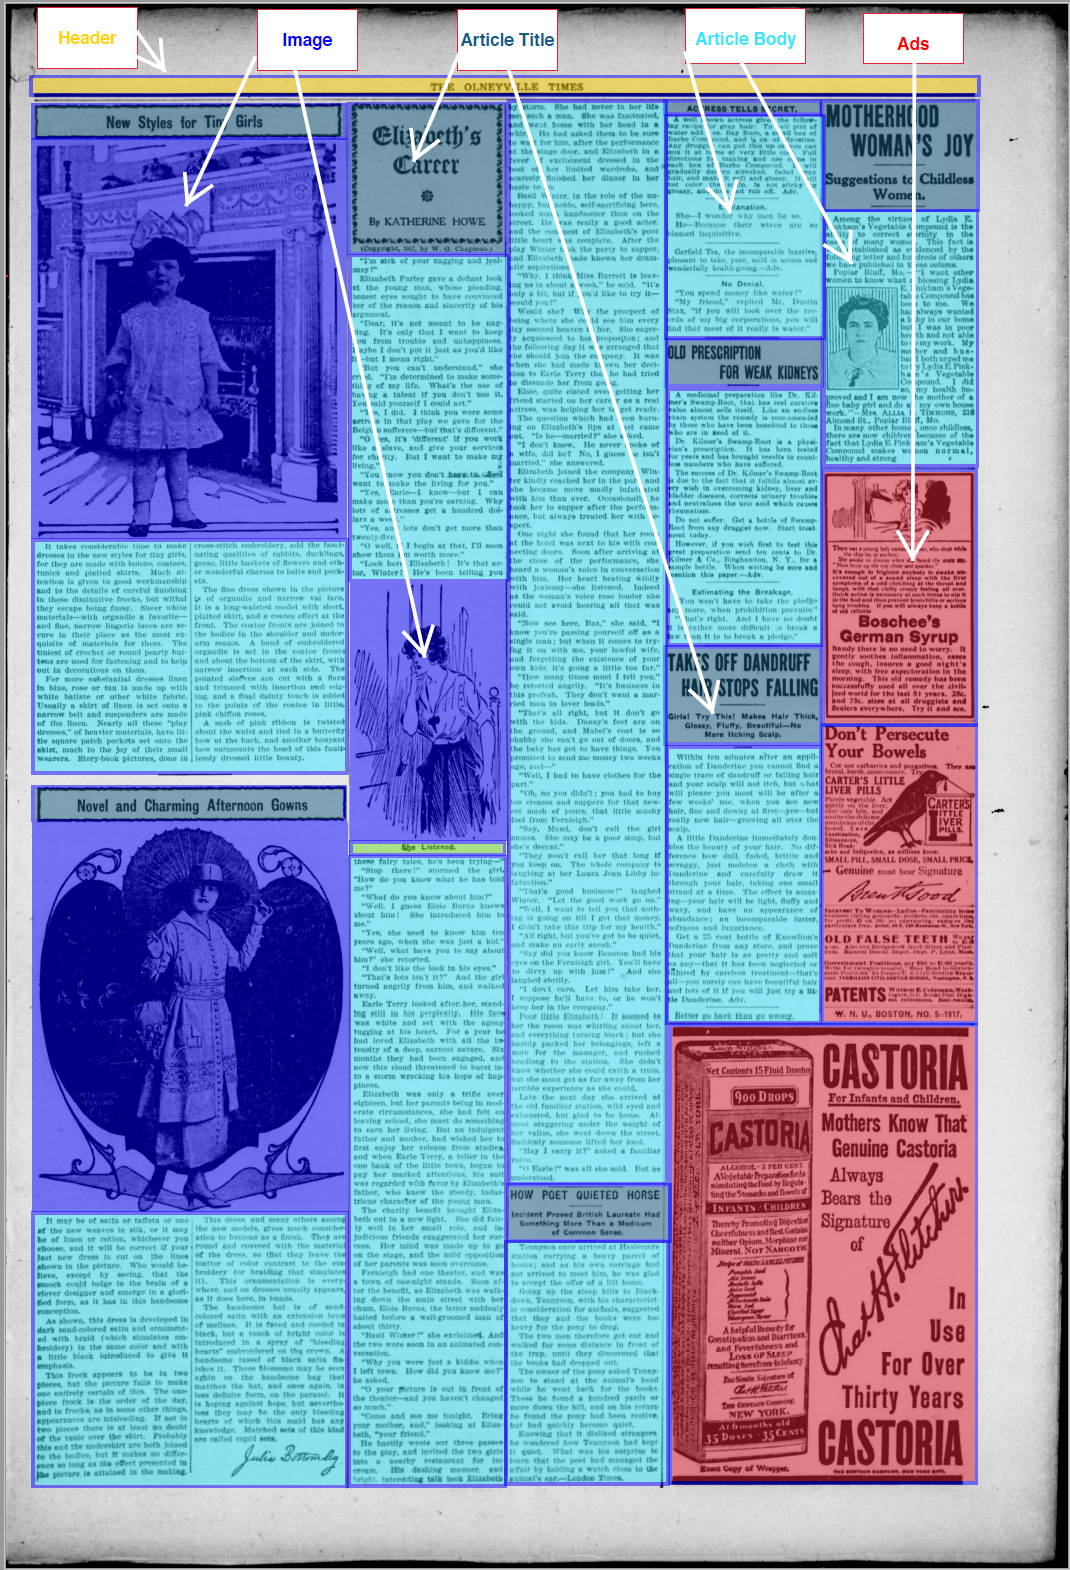
\includegraphics[scale=0.3]{LaTeX/Figures/labeling_example.png}
%   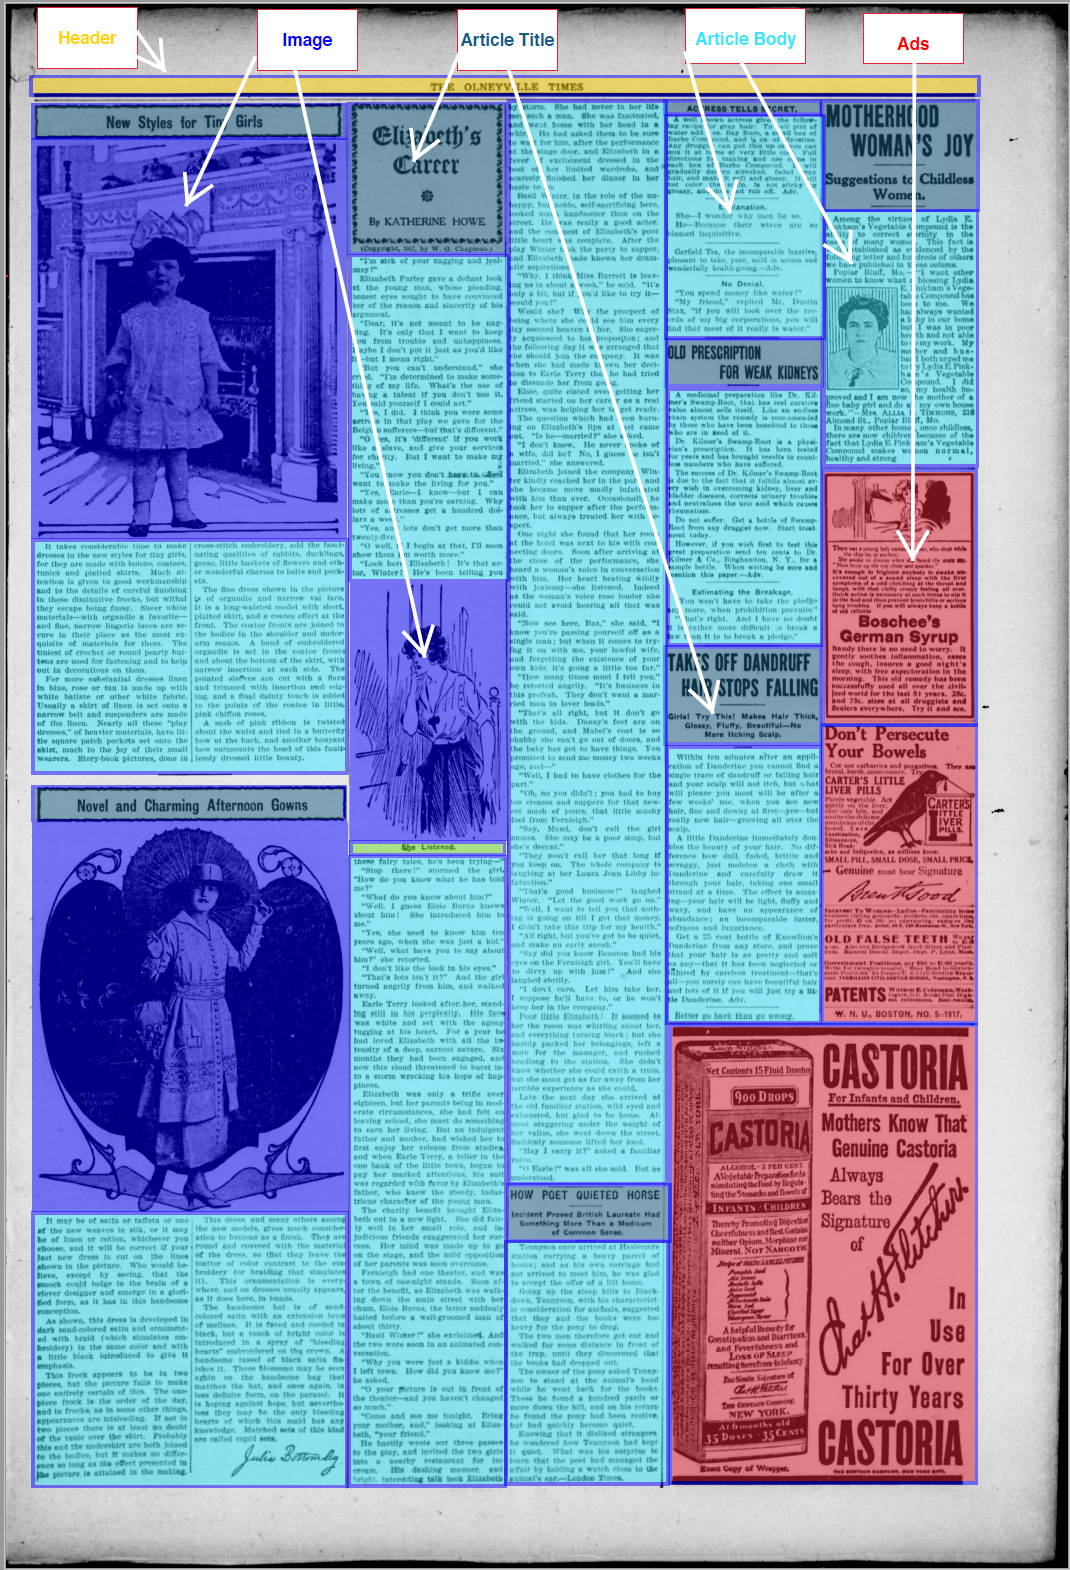
\includegraphics[width=\linewidth]{LaTeX/Figures/labeling_example.png}
  \caption{Example of Labeling Spec of NewsNet7 Dataset}
  \label{fig:NewspaperNet15}
 \end{figure}
    

\begin{table}[h]
\centering
% \scriptsize
% \captionsetup{font=scriptsize}
\small
\captionsetup{font=small}
\label{NewsNet7_data_stats}

\begin{tabular}{c|ccc}
\toprule
\multicolumn{1}{l}{}   & \multicolumn{3}{c}{\textbf{Number of instances}} \\ \hline
\textbf{Categories}    & \textbf{Train}  & \textbf{Test} & \textbf{Total} \\ \hline
\textbf{image}         & 10,017           & 1,793          & 11,810          \\
\textbf{article title} & 43,707           & 7,849          & 51,556          \\
\textbf{article body}  & 47,333           & 8,434          & 55,767          \\
\textbf{advertisement} & 35,165           & 6,228          & 41,393          \\
\textbf{table}         & 4,589            & 929            & 5,518           \\
\textbf{header}        & 1,930            & 343            & 2,273           \\
\textbf{other}         & 1,038            & 153            & 1,191           \\
\textbf{total}         & 143,779          & 25,729         & 169,508         \\
\bottomrule
\end{tabular}
\caption{NewsNet7 Dataset Statistics }
\end{table}

%From observation, almost all the documents we have seen can be fit into a rectangles, hence to fit into common object detection task. %We also convert the PRImA dataset from Polygon representation to the bounding boxes representation. (Is this needed?)

%The Amazon DocNet dataset contains 7 common object categories with x of them having more than y labeled instances, Fig. (insert here). In total the dataset has xxx labled instances in yyy images. In contrast to the PRImA datasets, Amazon DocNet has fewer categories but more instances per category. This can aid in learning detailed object models capable of precise 2D localization. 

\paragraph{RDCL2019 (ICDAR2019 Competition on Recognition of Documents with Complex Layouts)}
The NewsNet7 dataset does not include a text ground truth which requires an extensive manual labor. In order to evaluate the impact of the layout segmentation algorithms on the downstream OCR results, the RDCL2019 layout analysis dataset's \cite{DBLP:conf/icdar/ClausnerAP19} example set  is used, which includes 15 representative images with ground truth elements in XML format. It is important to note that these images are from contemporary documents such as magazines and they are only used to evaluate OCR performance. However, considering the fact that the layouts of these images are very different from historical newspapers, applying page segmentation models on this dataset as part of the process to obtain OCR results helps to assess their generalization capability.    
 
%------------------------------------------------------------------------

%-------------------------------------------------------------------------
%\begin{figure*}[h]
%   \centering
%   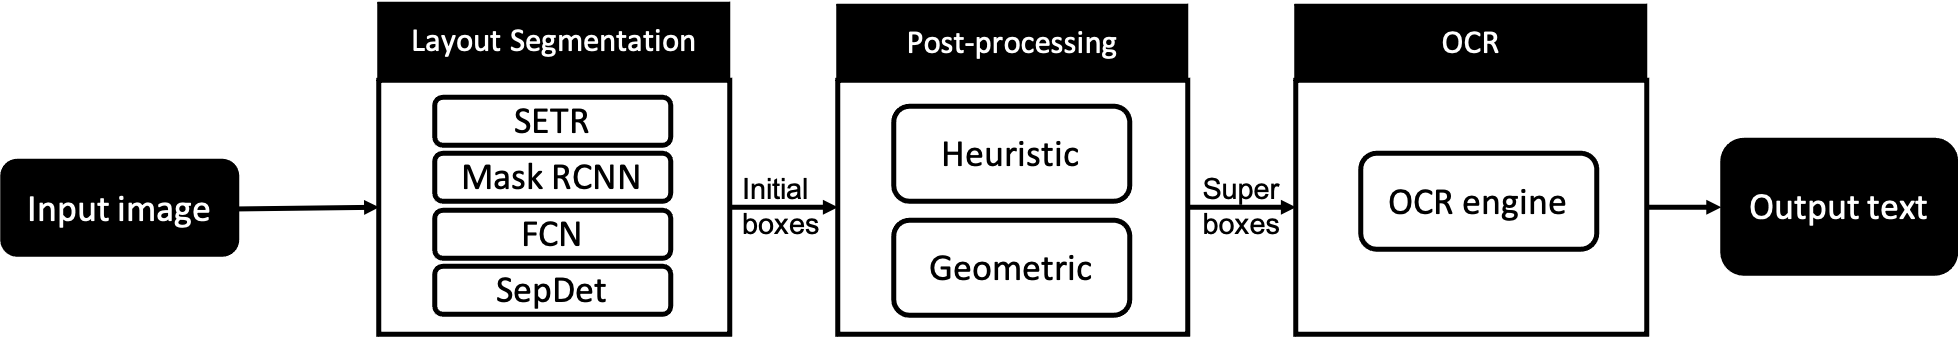
\includegraphics[width=\linewidth]{LaTeX/Figures/block_diagram_v3.png}
%   \caption{A pipeline from input image to output read-order OCR, where multiple layout segmentation and post-processing methods are explored.}
%   \label{fig:block_diagram}
% \end{figure*}
 

\section{Newspaper Digitization Methods}
The overall system architecture is illustrated in Figure \ref{fig:block_diagram} and can be summarized as follows. First, the input is an image of a document of arbitrary size, which is down-sampled to a fixed dimension and one of the listed document layout segmentation methods is applied to produce a segmentation map. Next, one of the listed post-processing methods is applied to convert the segmentation map to initial bounding boxes, then combined and ordered into super boxes. Finally, the super boxes are used to crop the image into manageable, high resolution blocks that are passed to an OCR engine to extract the text and the order of the super boxes are used to produce human read-order text for the entire document.

%The overall system architecture is illustrated in Figure \ref{fig:block_diagram} and can be summarized as follows: the input is an image of a document of arbitrary size, which is down-sampled to a fixed dimension; one of the listed layout segmentation methods is applied to a produce page segmentation map.
%% initial bounding boxes of content areas in the document;
%then one of the listed post-processing methods is applied to first convert the segmentation map to initial bounding boxes and then combine and order initial bounding boxes into super boxes; the super boxes are used to crop the image into manageable, high resolution blocks that are passed to an OCR engine to extract the text; finally, the super boxes and the corresponding extracted text are used in conjunction to produce human read-order text for the entire document.

\begin{figure}[h]
   \centering
%   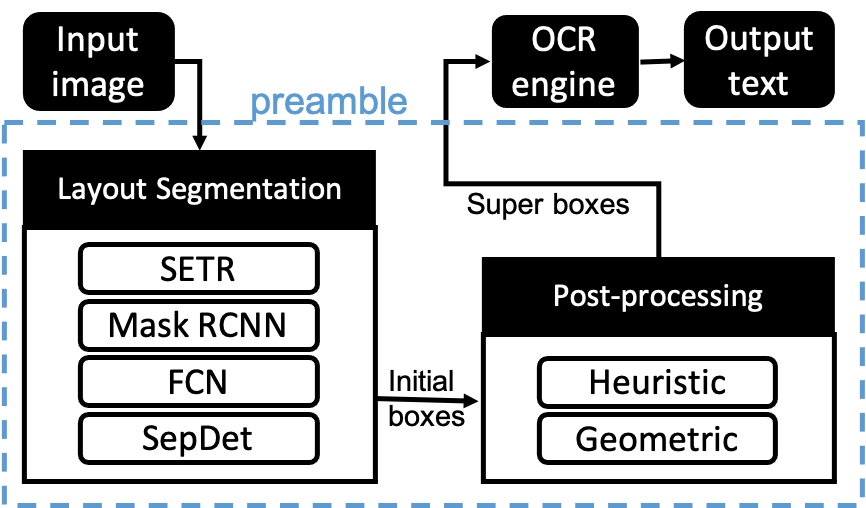
\includegraphics[width=\linewidth]{LaTeX/Figures/block_diagram_v5.png}
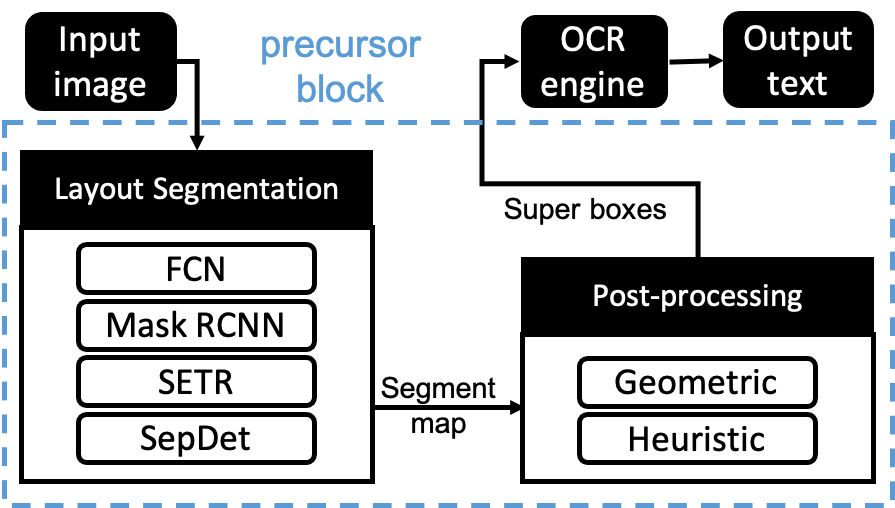
\includegraphics[scale=0.45]{LaTeX/Figures/block_diagram_v7.png}
   \caption{The framework pipeline}
   \label{fig:block_diagram}
 \end{figure}
 
\subsection{Document Layout Segmentation}
This section describes three different deep neural network architectures that are explored for document layout segmentation: Fully Convolutional Network (FCN), Mask R-CNN, and segmentation transformer (SETR). Figure \ref{fig:all_vis} shows the output of these models on a test newspaper image example.
% A later section on experimental setup will describe how these architectures will be paired with a set of ground truth to produce different types of output segmentation (e.g. two-class versus 7-class).



\subsubsection{FCN}
Inspired by a related study \cite{DBLP:conf/icdar/MeierSSAC17} that performs semantic segmentation approach based on the visual appearance of the document, the FCN semantic segmentation model is re-implemented in this work as a baseline. The fully convolutional neural network includes feature extraction, down-sampling convolution, upscaling deconvolution, refinement convolution, and a classification layer that classifies the pixels into classes. The model is trained from scratch with random weights initialization.

%The detailed network architecture is shown in the following figure (the refinement blocks aren’t shown given the size limit). 
In the last layer of the model, two different class settings are considered for pixel classification: seven-class setting that considers each of the semantic content types (i.e. header, article title, article body, image, ad, table) as separate classes and two-class setting that only regards foreground and background classes where foreground class includes all of the six content types; these settings are referred to as FCN-7 and FCN-2, respectively. 
% two sets of classes are considered: two-class and seven-class. For the two-class classification task, all of the content blocks (i.e. header, article title, article body, image, ad, table) are grouped together as foreground and other regions are treated as background. In order to have better separation of foreground versus background, the annotated bounding boxes were shrunk by a few percentages in all direction. For the seven-class classification task, each of the content blocks make up six of the classes, and the seventh class is made of anything not belonging to the content blocks and including the "other" class. 
The input images and the ground-truth masks are resized to 512 x 512 during the pre-processing steps
% Two sets of masks, two-class mask and seven-class mask, are generated for every sample from the ground truth bounding boxes of labeled segments. The images and corresponding masks were resized to 512 x 512 
and they are randomly combined into batches of 20 samples to be fed into the neural network. A weighted cross entropy loss is applied to better address and minimize the effects of class imbalance on the model. The FCN model is trained for 100 epochs with 2550 images, which takes almost 6 hours on a single GPU.

%The output of the FCN model is a pixel-wise probability map. Since the boundary of each segment is not a rectangle and cannot be readily used to crop the newspaper image for OCR analysis down the pipeline, multiple post-processing steps including some morphology-based algorithms are applied to convert the masks into a series of properly shaped and ordered bounding boxes before making calls to the OCR engine.
%%%%%%
% The FCN model for two-class (i.e foreground versus background) has same specifications as the SepDet model. 
% For the seven-class FCN model, the only difference is the training time was almost 6 hours for 100 epochs with 2550 images and inference is ms per image.

%%%%%%% ngnsl summarized the paragraph below since it will be repeated in post-processing section
% a morphology-based algorithm is used to convert masks into regions. More specifically, create binarized masks based on probability score of background versus non-background class, apply morphological operations (e.g. dilation and erosion) on the binarized image, apply a flood fill algorithm to build connected components, and get the bounding boxes for each connected component by finding the minimum and maximum of x and y coordinates. Once these small segments are obtained, a series of post-processing steps are applied before making calls to the OCR engine.
%%%%%%%%%%%%%%%%%%%%%%%%%%%%
%, as illustrated in the following figure.

%As part of feature extraction, the information in an image can be captured and encoded through convolution and max pooling. Then the deconvolution network decodes the downsized image and upscales it back to the original size. Finally, we applied a sigmoid function to make a pixel-level classification with probabilities.


% \begin{figure}[h]
%   \centering
%   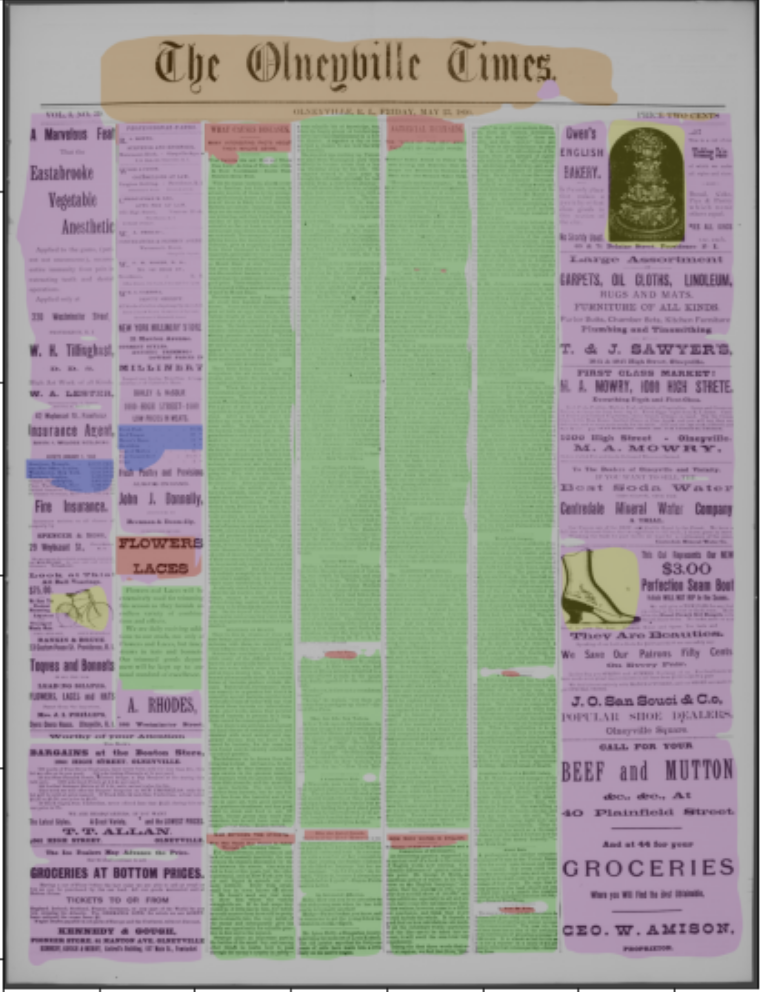
\includegraphics[width=\linewidth]{LaTeX/Figures/example_SETR.png}
%   \caption{An Example of the SETR model's predicted layout segmentation map for a newspaper image}
%   \label{fig:NewspaperNet15}
%  \end{figure}

\begin{figure*}[h]
   \centering
   \includegraphics[width=\linewidth]{LaTeX/Figures/work.pdf}
   \caption{Comparison of example page layout segmentation results}
   \label{fig:all_vis}
 \end{figure*}

\subsubsection{Mask R-CNN}
% Since for a given newspaper page, the OCR engine's direct input is a set of multiple cropped image segments and our NewsNet-7 is designed to represent each region as a rectangle, cropping a document with respect to its layout is naturally an instance segmentation problem. 
% The final bounding boxes could be disastrous when two adjacent column regions sharing a few connected pixels and it's not easy to disconnect them with morphological operations for it's rule-based method, meaning the parameters are correlated with the image resolution and pixel intensities. Hence, we natually adopted 
Mask R-CNN ~\cite{DBLP:conf/iccv/HeGDG17} is a widely-used state-of-art approach for instance segmentation. Since Mask R-CNN model predicts both bounding-boxes and semantic mask, it will saves us a considerable extra effort to obtain bounding boxes for OCR engine. And all the rest segmentation methods discussed in this paper require morphological process and labeling components to convert the semantic mask into bounding boxes. Moreover, the semantic mask from Mask R-CNN could be either polygon, which would also work for layout contains more complex shape that could not be represented by rectangles.
The Detectron2 framework ~\cite{wu2019detectron2} provides a large collection of baseline models including Mask R-CNN that makes experimenting with this model a fast and friction-less process.

In this work, two different backbone structures are used in the architecture of Mask R-CNN: the first backbone is a Residual Networks (ResNet) combined with a feature pyramid network (FPN) structure that uses standard convolutional and fully connected heads for feature extraction. The second structure, Dilated-C5 (DC5), is a ResNet conv5 backbone with dilation in conv5 and convolutional and fully connected heads for mask and bounding box prediction, respectively.
Moreover, for the ResNet component both ResNet-50 and ResNet-101 structures are used. Therefore, three different backbones are explored with Mask R-CNN, 
%we experiment with three different backbones for Mask R-CNN, 
which are R50-FPN, R101-FPN, and R50-DC5. The backbones are initialized with Microsoft Research Asia's original models trained on COCO \cite{DBLP:conf/eccv/LinMBHPRDZ14} dataset. 

The input images are resized such that their shorter sides are 800 pixels. The models are trained with a mini-batch of 2 images per GPU. The model with R101-FPN backbone is trained on 4 GPUs for 800 epochs, and the ones with R50-FPN and R50-DC backbones are trained on 8 GPUs for 1000 and 600 epochs, respectively. With this training setup, each experiment takes around 3-4 days. The learning rate is set to 3e-4 for all of the experiments. 
% Since from our observation, the article title usually is extremely small, especially when being compared with the overall page (\textasciitilde 7k x 10k about 70 million pixels per page on average). Therefore, in order to not to miss any small objects, we selected 1024 RoI heads per image instead of the default 512.

% Note that the Mask R-CNN output is instance segmentation, the results is not directly a semantic mask, hence needs to be post-processed to be able to compare with other semantic models. For each predicted instance, we have a binary mask to represent the segmented polygons. We also used self-defined priority class when doing mask conversion. For instance, it is very common that a table is within an advertisement, or an image is within an article. In order to solve the class conflicts when there is an ``overlapping'' on a pixel, we ranked the classes in a way such that the priority is image $>$ table $>$ article title $>$ header $>$ advertisement $>$ article body $>$ other. Moreover, another way to construct the predicted mask is to dump the predicted mask and rasterize the predicted bounding-boxes the same way we rasterize the bounding boxes when making the groundtruth mask. Intuitively, rasterization from bounding boxes would bring up the benchmark metrics significantly but due to time limit, we don't have enough time to compare these two methods.


% A placeholder for output converter, comvert the instance into semantic mask with customized priorities of each mask.

%  \begin{figure}[ht]
%   \centering
%   \includegraphics[width=\linewidth]{LaTeX/Figures/sn92064044_1890-05-23_ed-1_seq-1.png}
%   \caption{MaskRCNN Results on NewspaperNet test set - a zoom-in example}
%   \label{fig:NewspaperNet15}
%  \end{figure}
 
%  \begin{figure}[ht]
%   \centering
%   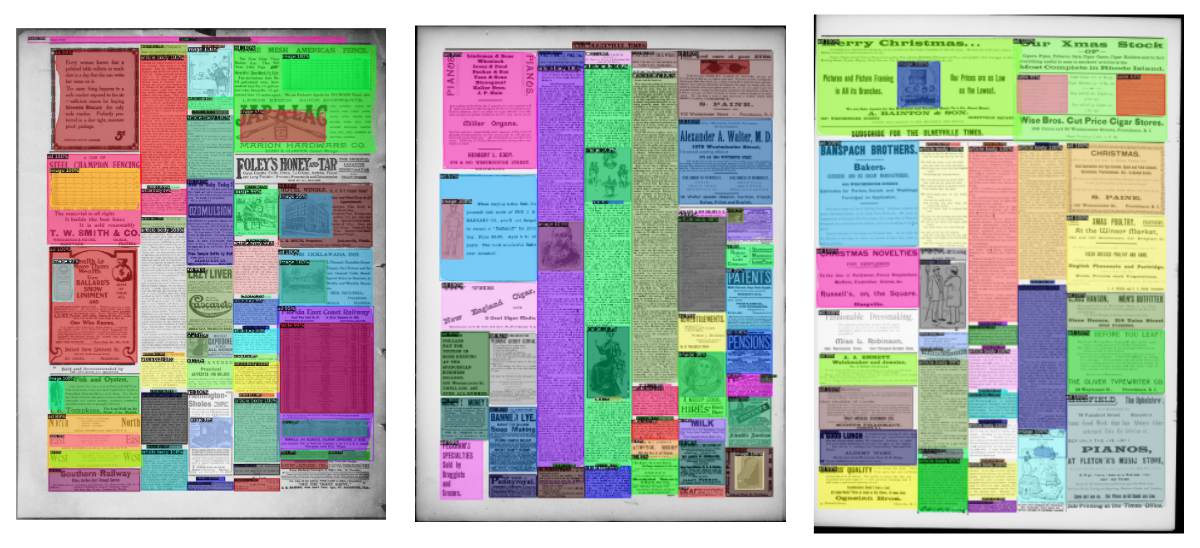
\includegraphics[width=\linewidth]{LaTeX/Figures/newspaper3.png}
%   \caption{MaskRCNN Results on NewspaperNet test set. These results are based on ResNet-101, achieving a mask AP of 49.2. Masks are shown in color, and bounding box, category, and confidences are also shown}
%   \label{fig:NewspaperNet3}
%  \end{figure}

% Futhermore, Mask R-CNN also shows amazing generalization on RDCL2019 dataset \cite{DBLP:conf/icdar/ClausnerADP19}, see Figure \ref{fig:rdcl19} in Appendix for reference.
 
 
\subsubsection{SETR}
The Segmentation transformer (SETR) model (Zheng et al. 2021) has been recently shown to achieve the state of the art results in semantic segmentation on a number of datasets including ADE20K and Pascal Context.

What makes SETR different from the previous segmentation models with fully convolution encoder-decoder structures is that it reformulates the task of semantic segmentation from a sequence to sequence point of view. Following this intuition, it considers semantic segmentation task as translating an input image into a probability density map with the same resolution and employs an architecture similar to language translation models to tackle the problem.

To convert an input image into a sequence, it is divided into a grid of fixed-size patches. Each patch is then flattened and linearly projected into an embedding space.  After adding positional encoding to the embedded vectors, they are fed to a transformer encoder that outputs a sequence of feature maps. Finally, a simple convolution decoder followed by some upsampling operations is applied to the feature maps to convert them to the original image resolution.

% What results in a performance boost for this model compared to the previous fully convolutional models is that it addresses the problem of limited receptive field in these models by modelling global context in every single layer of the encoder using a transformer structure.

In our experiments with the SETR model, multiple different augmentation techniques such as random-cropping, random-resizing and flipping were used to make the training more robust to over-fitting. Moreover, 
% since in the input images the distribution of pixels over different output classes was not balanced,  
a weighted cross-entropy loss is used for optimization to compensate for the class imbalance in input pixel distributions.
% This loss weights the computed loss for pixels from different classes differently.
The model is trained with a batch size of 2 images for 1000 epochs. The input resolution is set to 512x512 pixels to allow training on a single GPU. The initial learning rate is set to 0.001 and it is decayed with a rate of 0.999 after every epoch. Under the above setting, training this model takes about 5 hours.
% The average inference time of the model is about 350 ms per image.\\

A series of heuristic post processing steps are applied to prepare the model's output for the next steps down the pipeline which will be explained in the next section.


\subsubsection{SepDet}
Instead of putting the model focus on the entities that need to be digitized, a new deep neural net based model that followed the idea behind classic top-down approach  was proposed and experimented. The new Separator Detector (SepDet) model was developed to detect separators (e.g. lines or white spaces that separate different articles or multiple columns of a single article) that exist in the documents. These separators are very useful for layout analysis as they contain important information to identify the logical structure of a newspaper page. The purpose of this model is to separate the text regions from the background and split them into a series of logical blocks using detected separators. Instead of using heuristics to identify the locations of these separators, a FCN model is trained to do such task.  As the model name indicates, this model does not differentiate different entity types (e.g. table, ad and articles) among the text regions. For this model, the ground truth only contains 2 classes: separators and non-separators.  To accelerate training while maintaining enough details for detecting the separators, the original input images are scaled to 512x512 pixels. As these separators often comprise less than 10 percent of the image area, a weighted cross-entropy loss is implemented for training the model. 
% The predicted mask are passed through a series of post-processing steps to generate ordered bounding boxes that are ready to be used for cropping the images prior to OCR API call.
% After getting the generated mask from the FCN model, similar steps (i.e. binarization and finding connected components) are followed to convert the masks to segments. However, since the separators are more clear in the output of SepDet model, it's easier and more effective to get good segments without sophisticated post-processing.\\
In our experiments with SepDet model, it is trained using a mini-batch size of 20 images for 100 epochs. The learning rate is set to 0.0005. With 2550 training images, it takes 1 hour and 20 minutes to train the model on a single GPU.
% For inference, this model runs at 262ms per image on an NVIDIA V100 Tensor Core GPU. \\
A visualization of the predicted separators by SepDet for a test image and the corresponding processed ground truth map are shown in Figure \ref{fig:SepDetmodelPred}.
%Visualizations of the segments for the newspaper and magazine test cases are provided in Figure \ref{fig:SepDetmodelNewspaper} and Figure \ref{fig:SepDetmodelMag}. 
\begin{figure}[ht]%
\centering
\subfloat[\centering Predicted separators ]{{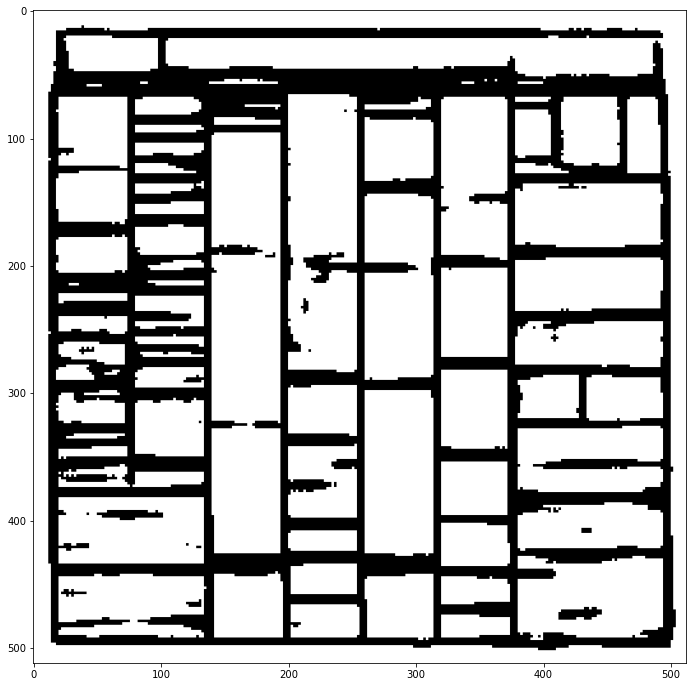
\includegraphics[width=.4\linewidth]{LaTeX/Figures/sn92064044_1890-05-23_ed-1_seq-1_mask_predicted.png} }}%
\qquad
\subfloat[\centering Ground truth of the separators ]{{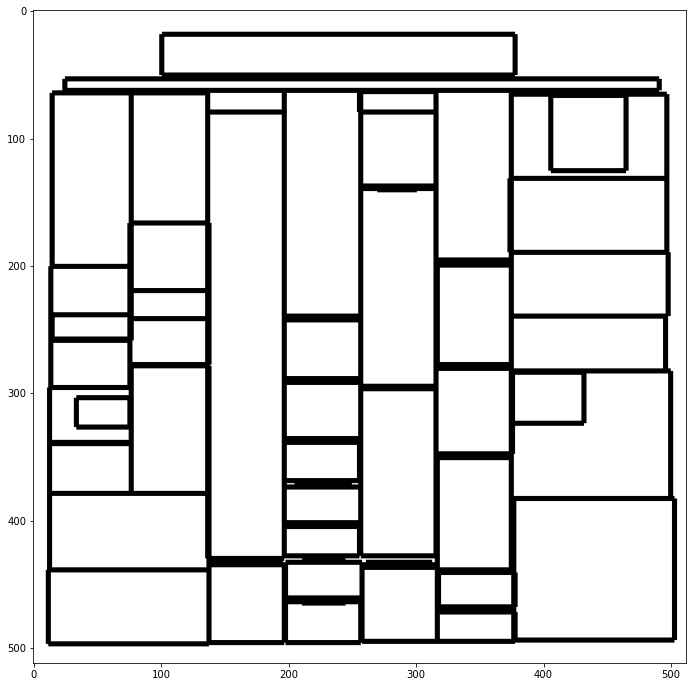
\includegraphics[width=.4\linewidth]{LaTeX/Figures/sn92064044_1890-05-23_ed-1_seq-1_gt.png} }}%
\caption{Predicted separators compared with ground truth}%
\label{fig:SepDetmodelPred}%
%   \centering
%   \includegraphics[width=\linewidth]{LaTeX/Figures/sn92064044_1893-06-30_ed-1_seq-7.png}
%   \caption{Left:}
%   \label{fig:SepDetmodelPred}
\end{figure}

%  \begin{figure}[ht]
%   \centering
%   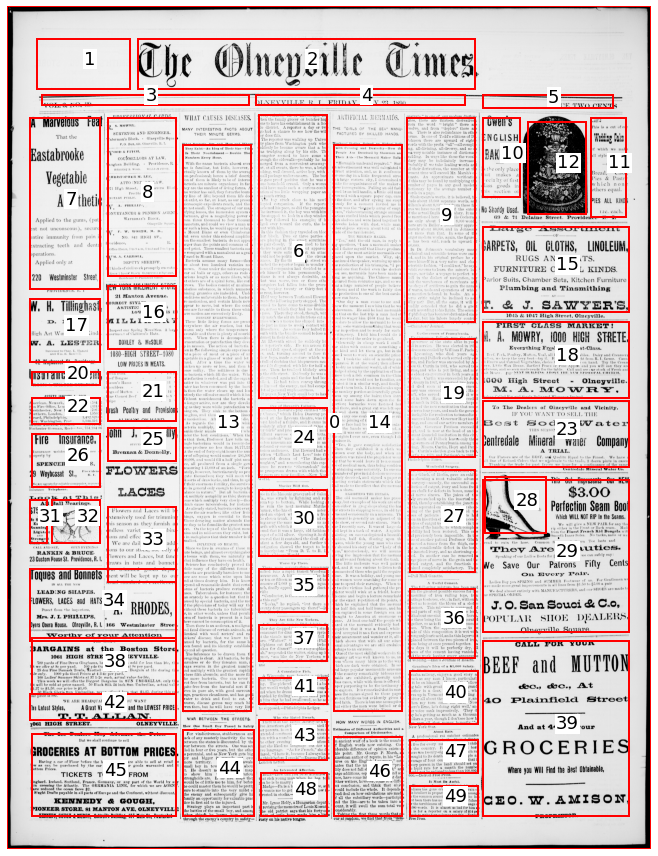
\includegraphics[width=\linewidth]{LaTeX/Figures/test_2_segments_sep_weight_3.png}
%   \caption{SepDet segmentation results on NewspaperNet test set. The order of the segments is based on simple heuristics (i.e. top to bottom, left to right). }
%   \label{fig:SepDetmodelNewspaper}
%  \end{figure}

%  \begin{figure}[ht]
%   \centering
%   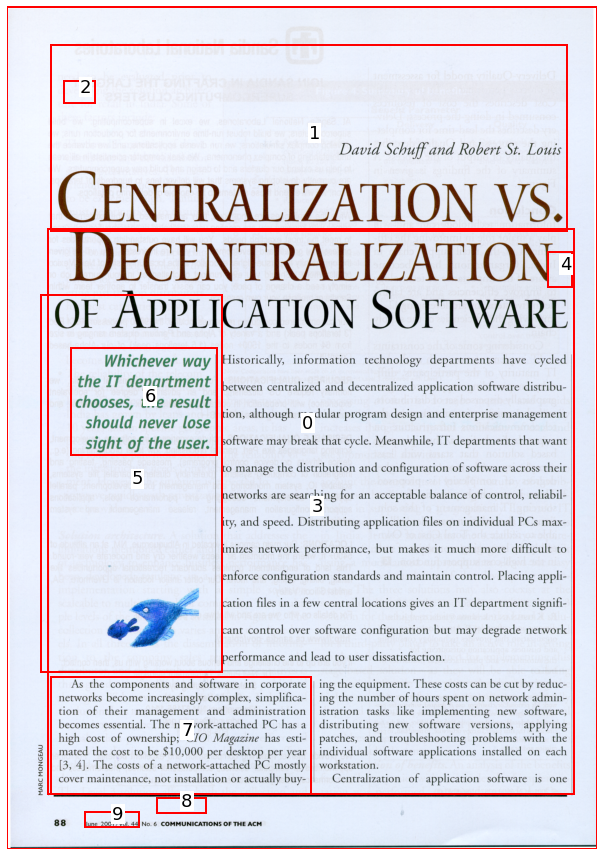
\includegraphics[width=\linewidth]{LaTeX/Figures/00770085-segments-predicted.png}
%   \caption{SepDet segmentation results on RDCL2019 test set - a magazine example. The order of the segments is based on simple heuristics (i.e. top to bottom, left to right). }
%   \label{fig:SepDetmodelMag}
%  \end{figure}

\subsection{Post-processing methods}

In this section, two post-processing strategies are introduced. These techniques convert the output of a segmentation model to a series of bounding boxes with a format that is proper for the OCR engine.

\subsubsection{Geometric}
% Geometric algorithms are commonly used for solving geometric input and output problems, hence, for the post-processing, intuitively, 
In this post-processing technique, bounding boxes are computed and refined in the following two steps.
% we adopted classical morphological operations and flooding algorithm to find connected components that can be used to convert segmentation masks to bounding boxes. 
% In this section, we list several geometric problems encountered as part of this process and present solutions for tacking each of them.
%%%
% \paragraph {Converting a segmentation map to bounding boxes}
This first step is extracting bounding boxes from a predicted 2D array that represents class probability distribution over pixels.
% Given a 2D array representation of a semantic mask where each pixel represents the class probability distribution for that pixel over all class, compute the bounding boxes for such a mask.
To tackle this task, first the Ostu's thresholding method (N. Otsu 1979) is applied to convert the probability map as an grayscale mask into a binary mask.
% Though we can apply \textbf{morphological operator} directly on grayscale images, a more common approach is still to use an auto-thresholding algorithm such as Ostu's algorithm (N. Otsu 1979) to convert the given grayscale mask into a binary mask.
After that opening morphology operation is applied to eliminate small regions in multiple iterations.
% (3 iterations with 3x3 square kernel and 14 iterations with 3x3 horizontal kernel).
% After experimenting with structuring element shape and size, we finally limited to 2 kernels, which are classical square-shaped 3x3 element and horizontal-shaped 3x3 element. 
% In the second step, in order to filter out small connected components, we applied open operation on binarized image with square-shaped 3x3 element for 3 iterations, then applied open operation with  horizontal-shaped 3x3 element for 14 iterations. 
Next, the flooding algorithm is applied to label all of the connected components distinctively. Finally a bounding box is fitted to each refined connected component. Figure \ref{fig:mask2bbox} illustrates the explained process.
% by computing the horizontal and vertical range over which the component is spanned.

% After we obtained the smoothed connected components, we then will use the flooding algorithm to label all the connected components and assign distinct labels on each ``island''. Lastly, for each labeled mask, we find its instance's minimum and maximum coordinates to locate the bounding boxes $(x_{min}, y_{min}, x_{max}, y_{max})$. 
% Figure \ref{fig:mask2bbox} illustrates different steps of this process. Further implementation details along with a pseudocode are presented in the Appendix section.

 \begin{figure}[t]
   \centering
   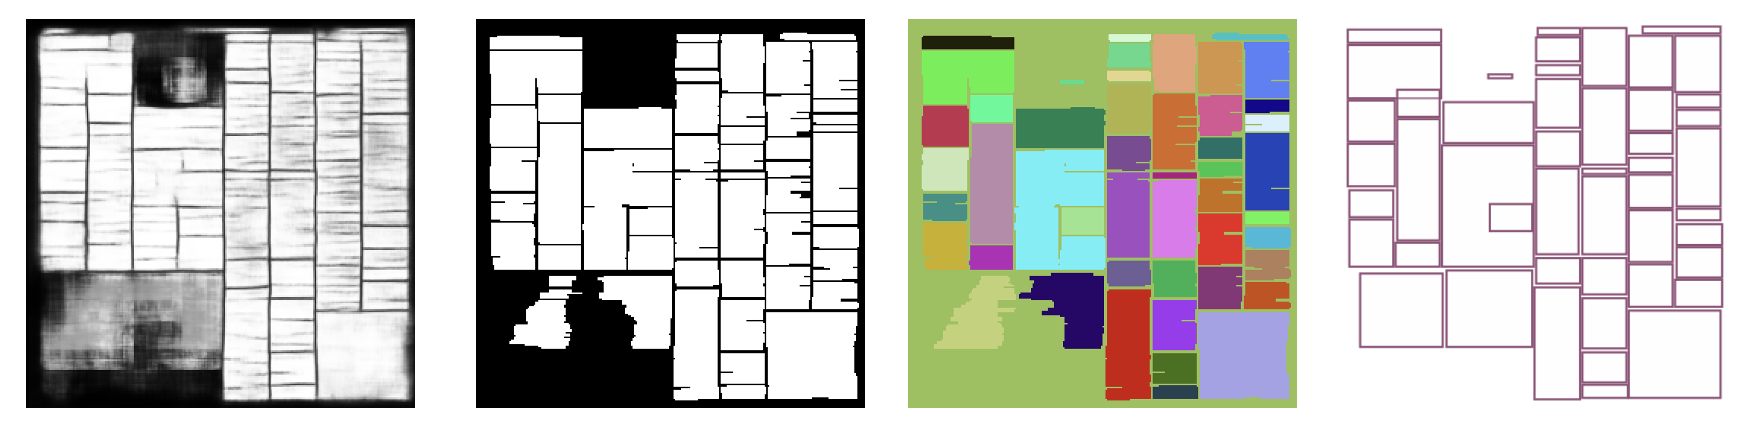
\includegraphics[width=\linewidth]{LaTeX/Figures/mask_to_bbox.png}
   \caption{Illustration of the 4 steps to convert a semantic mask to bounding boxes, from left to right are original grayscale FCN-2 mask, binarized mask with morphological operations, connected components, and final bounding boxes}
   \label{fig:mask2bbox}
 \end{figure}
 
%%%
% \paragraph {Removing gaps between bounding boxes}
The second step is removing gaps between bounding boxes.
%We noticed there are 
There are often small gaps of several pixels between boundaries of annotated segments in the ground truth when the text columns are very close.  Since the models are trained on down-sized ground-truth,  when up scaling the bounding boxes to original scale, those gaps can be inflated, resulting in missing text characters near the boundaries. 
To reduce those gaps, the predicted bounding boxes were expanded by applying 
%We took measures to reduce those gaps by expanding the predicted bounding boxes. 
%More specifically, we applied 
a clustering algorithm (Figure \ref{fig:character_loss}) on bounding box vertices to replace the neighboring vertices with each cluster's centroid.

% From our experiments, we find out in almost all semantic segmentation methods will produce masks with gaps. A reasonable guess is when the mask is significantly down-sampled from the original image, it is common that the post-processed bounding-boxes have gaps when scale back to original image size by multiplying the ratio. An easy calculation here - original image width and height is usually 7kx10k pixels, resizing it to 512x512 make a mask 13-20 times smaller on the Newspaper's width and height. Hence for every single single pixel difference, it would become 13-20 pixels gap. From eye-balling many visualizations, Mask R-CNN don't suffer this problem due to it is producing bounding-boxes directly. Those gaps usually lead to ``character loss'' (see \ref{fig:character_loss}), which will penalize OCR accuracy in the later character recognition stage. In order to tackle this problem, we applied a clustering algorithm on bounding boxes vertices to replace the neighboring vertices with the cluster's centroid.

 \begin{figure}[h]
   \centering
   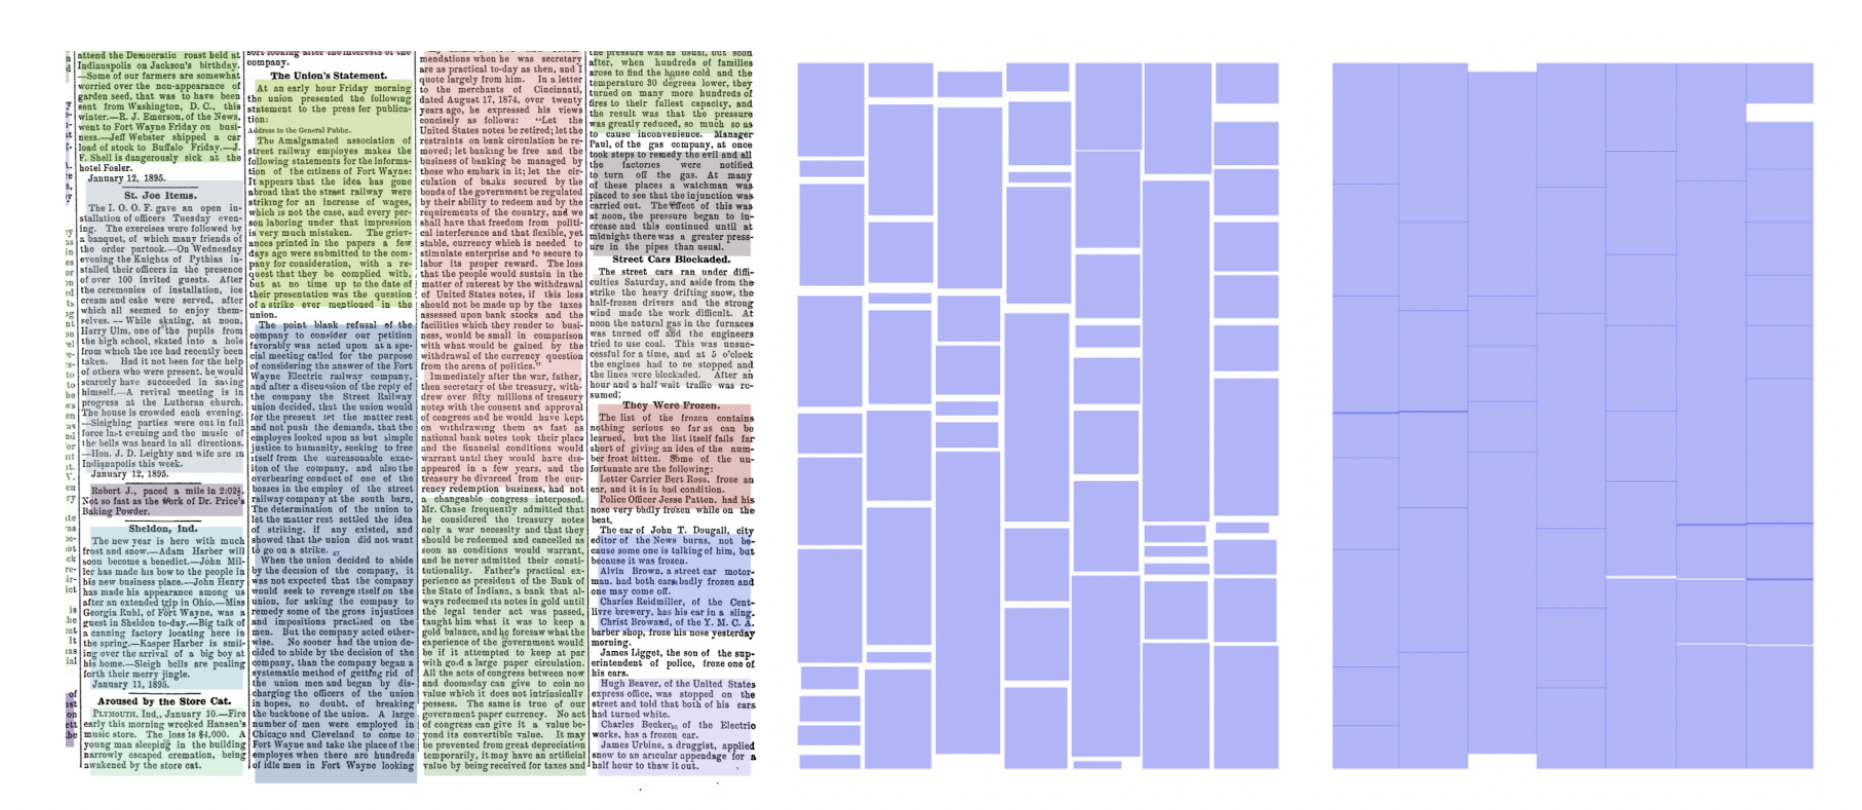
\includegraphics[width=\linewidth]{LaTeX/Figures/clustering_v.png}
   \caption{Left side: illustration of bounding boxes gap that will lead to character loss in OCR step; right side: illustration of clustering vertices operation.}
   \label{fig:character_loss}
 \end{figure}
 
% We utilized graph representations to model bounding boxes relations.

% \paragraph{Remove Overlapping Bounding-boxes}

% We first build an undirected weighted graph $G = (V, E)$, where $V = \{B_{1}, B_{2}, ..., B_{m}\}$ denotes a set of bounding boxes on an image,  and $E $ is the set of possible interconnections between pairs of bounding boxes. We define connection in the way such as if a pair of bounding boxes $(B_{i}, B_{j})$ intersect with each other, we add an edge $(i, j)$ in $E$, and for each edge $(i,j)\in E$ we have a weight $w(u,v)$ specifying the ratio of area of intersection over that pair. % I should add an visual to illustrate this.

% In this way, the overall page's bounding boxes can be represented as a graph, we then use union-find data structure to obtain the grouped nodes within $O(log(n))$ time, and for each grouped subgraph, we can examine each edge's weight and use the node to retrace the original bounding box, if the weight is greater than a certain threshold, such as 0.9, which indicates the 90\% of  the smaller bounding-boxes is completely within the larger neighbor. We then remove this bounding box from this page.  \\

%%%%%%%%%%
% In addition to the above, for the Mask R-CNN model, we also had to removed the overlapping bounding boxes in the post-processing step to both decrease the number of OCR API calls and avoid potential post OCR noise caused by redundant text. 
%%%%%%%%%%

% In the post processing steps we also removed overlapped bounding-boxes and merged regions that are vertically adjacent. The motivation of reducing the redundant bounding boxes is to reduce the number of API calls since in real-world application, our customers are in dire needs of time and cost efficiency. Besides, too many redundant bounding boxes in OCR stage would also introduce too much noises that produce repeated texts and increase the difficulty for OCR post-processing and XML reconstruction.

% After we combine all the geometric-based post-processing steps, the final bounding boxes we feed to OCR engine are significantly improved in both the shape and numbers of bounding boxes, please see Figure \ref{fig:pp} in Appendix for visualization.

%  \begin{figure}[h]
%   \centering
%   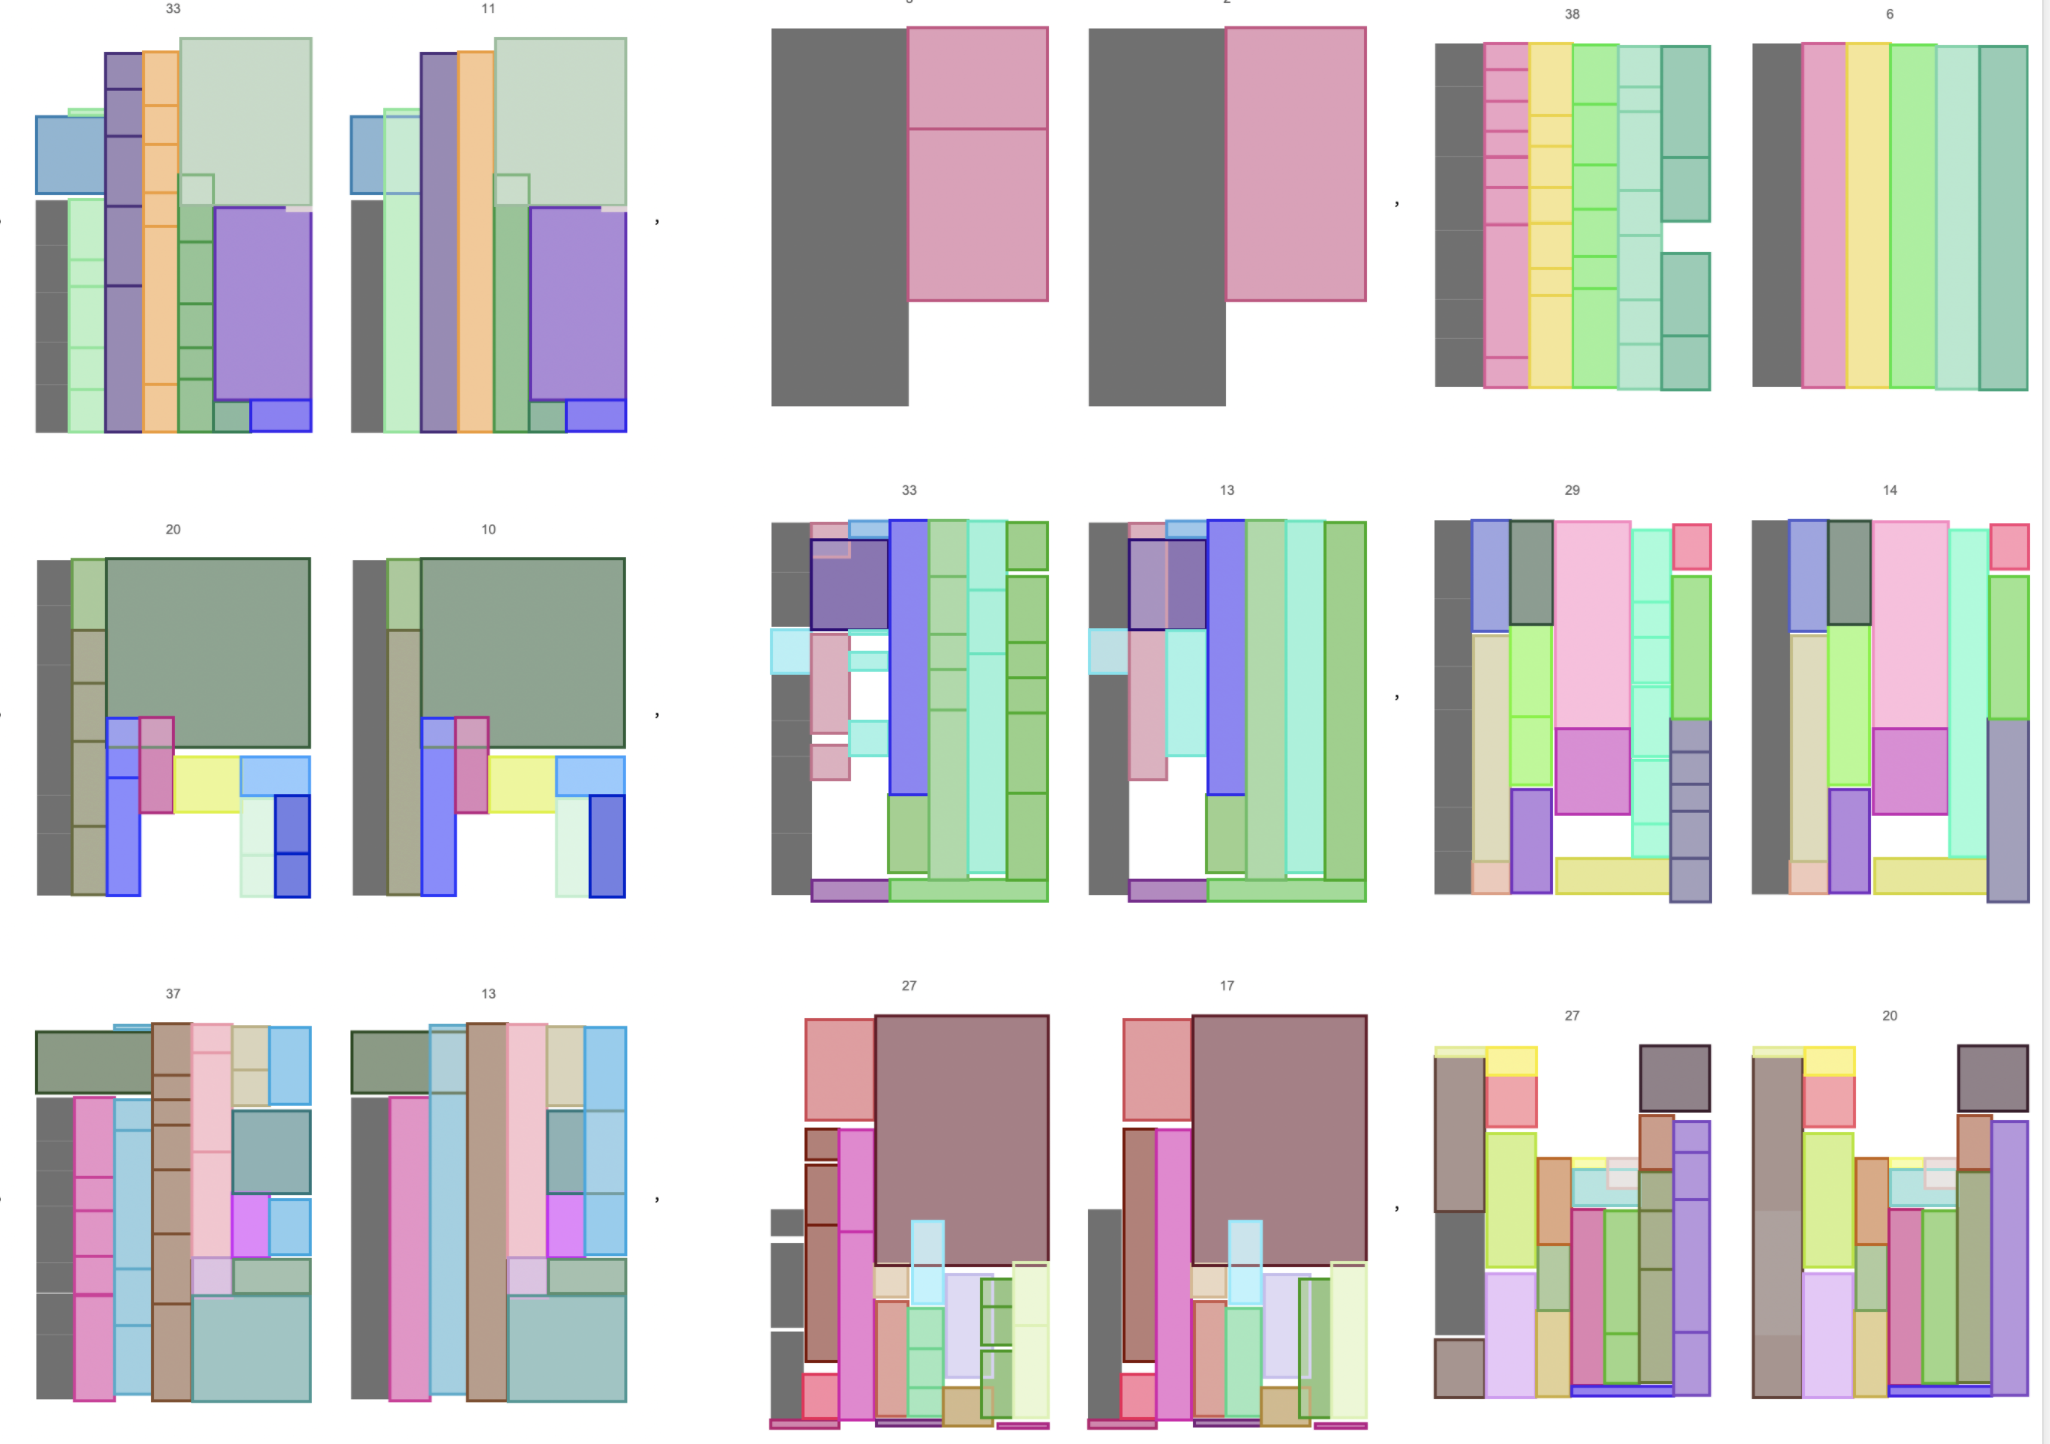
\includegraphics[width=\linewidth]{LaTeX/Figures/bbox_post.png}
%   \caption{Visualization of post-processing steps}
%   \label{fig:pp}
%  \end{figure}
 
%\paragraph{Vertical-Merging}


% \section{Experiment Setup}
\subsubsection{Heuristic}

This post-processing algorithm serves three main purposes. The first purpose is to convert the generated maps at the output of a segmentation model to bounding boxes. These bounding boxes are used to crop the input images around the text segments so that they can be digested by the OCR engine. The second purpose is to combine the generated bounding boxes by the previous step, whenever it is possible, to minimize the number calls to the OCR API for cost optimization. Finally, the last purpose is to logically order the final bounding boxes so that the final extracted text can be read in a right human readable order.

In order to accomplish the first purpose, similar techniques explained in the geometric post-processing approach are employed.
To accomplish the second purpose, bounding boxes that are vertically aligned with some tolerance threshold are combined together regardless of their class (as they are expected to be in the same column). Finally, in order to accomplish the third purpose, final combined bounding boxes are ordered from top left to bottom right to follow human reading habits.


%------------------------------------------------------------------------
\section{Experimental Results}
In this work two different types of evaluation experiments have been conducted: isolated layout segmentation evaluation and end-to-end OCR evaluation. For all the models, the checkpoint that corresponded to the best performance on the validation set was used for the experiments.
% For all of the experiments in this section, the models were trained on either single or multiple NVIDIA V100 Tensor Core GPU with 61 GiB of memory.\\
\subsection{Layout Segmentation Evaluation}

In order to asses the performance of the layout segmentation models, the predicted masks are evaluated using a series of pixel-wise metrics including mean Intersection over Union (mIoU), mean Accuracy (mAc), mean Recall (mRe), mean Precision (mPr) and mean Fscore (mFs). Each of these metrics was first evaluated for each class separately and then was averaged over all of the classes.

In the experiments, two different groups of models are considered, each with a different level of layout granularity. The first group of models which included, FCN-7, SETR and different types of Mask R-CNN models, were trained to differentiate between all of the 7 classes of layouts. The second group of models that included the SepDet and FCN-2 models were however blind to any layout granularity during training, which means they were trained to only differentiate between text and background pixels. The purpose of these experiments was to analyze how much having access to knowledge about different layout types can guide highly expressive models in the basic task of predicting text regions, which is the only required knowledge for OCR engine. Due to this training methodology difference, these two groups are compared separately on their segmentation performance. Table  \ref{table:layoutmetric_7c}  
% and Table \ref{table:layoutmetric_2c} 
shows the segmentation performances of the first and second groups.

% \subsubsection{Semantic Evaluation on 7 classes} ** just compare the results for the setr and maskrcnn when all of the numbers are available.
\begin{table}[h]
\scriptsize
\captionsetup{font=scriptsize}
\begin{tabular}{l|cccccc}
\toprule
\textbf{metrics}  & \textbf{mIoU} & \textbf{mAc} & \textbf{mPr}  & \textbf{mRe}  & \textbf{mFs} & \textbf{IT}\\
\hline
MaskRCNN-R101-FPN 	& 63.35 & 80.48 & 80.48 & 77.04 & 83.39 & 0.201\\ % will re-run experiments on the new resolution

MaskRCNN-R50-FPN  	& 63.90 & \textbf{80.66} & 80.66 & 77.45 & \textbf{83.82} & 0.152\\ % will re-run experiments on the new resolution

MaskRCNN-R50-DC5     	& 63.37 & 80.22 & 80.22 & 77.02 & 83.67 & \textbf{0.082}\\ % will re-run experiments on the new resolution

SETR              	& \textbf{70.02} & 80.14 & \textbf{86.13} & \textbf{80.28} & 82.80 & 0.345 \\

FCN-7 &  56.34 & 71.38 & 74.08  & 70.99 & 79.60 & 0.493\\
\hline
\hline
FCN-2    &  \textbf{76.97}   & \textbf{84.92}  & \textbf{90.68}  & 86.78   & \textbf{88.57} & 0.489  \\
SepDet          & 44.01 & 83.23 &  46.27  &  \textbf{90.02}  &   61.12  & 0.299\\
\bottomrule
\end{tabular}
%\caption{Layout segmentation metric for models that differentiate 7 classes in the annotations }
\caption{Layout segmentation performance for different segmentation models. \textbf{IT} in this table represents inference time in seconds on a single NVIDIA V100 GPU. Note that SepDet and FCN-2 are evaluated on 2-class setting (foreground/background).}
\label{table:layoutmetric_7c}
\end{table}

% \subsubsection{Semantic Evaluation on 2 classes}
% ** compare the results for sepdet and FCN here, when all of the numbers are available.\\
% As SepDet only aims to separate the text regions from the background into logical blocks using these separators, there are will be only 2 classes for the predicted pixel-level segmentation results. Metrics are reported in the Table \ref{table:layoutmetric_2c}. 

% \begin{table}[h]
% \small
% \begin{tabular}{l|ccccc}
% \toprule
% \textbf{metrics}  & \textbf{mIoU} & \textbf{mAc} & \textbf{mPr}  & \textbf{mRe}  & \textbf{mFs} \\
% \hline
% FCN-Morphology    &  84.58   & 88.57   & 98.00  & 86.06   & 91.64  \\
% \hline
% SepDet  &  44.01  &  83.23  &  46.27  &  90.02  &   61.12  \\
% \bottomrule
% \end{tabular}
% \caption{Layout segmentation metric for models that only differentiates foreground text regions and background}
% \label{table:layoutmetric_2c}
% \end{table}

%%%%%%%%%%%%%%%%%%%
% \begin{table}[h]
% \scriptsize
% \begin{tabular}{l|cccc}
% \toprule
% \textbf{Class}  & \textbf{\begin{tabular}[c]{@{}c@{}}mPr\\ SETR \end{tabular}} & \textbf{\begin{tabular}[c]{@{}c@{}}mPr\\ MaskRCNN \end{tabular} } & \textbf{\begin{tabular}[c]{@{}c@{}}mPr\\FCN
% \end{tabular}} & \textbf{\begin{tabular}[c]{@{}c@{}} AP(bbox)\\ MaskRCNN
% \end{tabular}} \\
% \hline

% Article-body 	& 92.98    & - & 93.07 & -\\

% Article-title   & 73.78    & - & 74.41 & -\\

% Ad    	        & 92.61    & - & 91.70 & -\\

% Image           & 81.22    & - & 53.55 & -\\

% Table           &  80.73   & - & 41.62 & -\\

% Header          &  85.72   & - & 75.78 & -\\
% \bottomrule
% \end{tabular}
% %\caption{Layout segmentation metric for models that differentiate 7 classes in the annotations }
% \caption{Per-class layout segmentation results for the set models that were trained with 7-classes granularity. For this experiment the {*}{R\_101\_FPN\_3x} backbone was used for MaskRCNN.}
% \label{table: perclass_layout_metrics}
% \end{table}
%%%%%%%%%%%%%%%%%


% \begin{table}[h]
% \scriptsize
% \centering
% \begin{tabular}{c|ccccc}
% \toprule
% \begin{tabular}[c]{@{}c@{}}Backbone \\ name\end{tabular} & \begin{tabular}[c]{@{}c@{}}box\\ AP\end{tabular} & \begin{tabular}[c]{@{}c@{}}mask\\ AP\end{tabular} & \begin{tabular}[c]{@{}c@{}}train \\ time \\ (s/iter)\end{tabular} & \begin{tabular}[c]{@{}c@{}}inference \\ time \\ (s/im)\end{tabular} \\ \hline
% R50-FPN   &       &       & 0.952  & 0.152 \\
% R101-FPN  & 49.2  & 49.4  & 1.256  & 0.201  \\
% R50-DC5   &       &       & 1.759  & 0.082 \\

% \bottomrule
% \end{tabular}
% \end{table}

When comparing the layout segmentation evaluation results from Table \ref{table:layoutmetric_7c}, it can be observed that the SETR and Mask R-CNN models perform very competitively in layout segmentation and they considerably outperform the FCN model. It can also be observed that among different versions of the Mask R-CNN model, the one with R50-FPN backbone outperforms the rest and its performance is fairly close to the SETR model. \\ Considering these observation while keeping the inference time of the models into account, the right choice of the model is highly dependent on the limitations of the use-case. For those use-cases where the target application heavily relies on accurate classification of layout segments, the SETR model and even the Mask R-CNN model with R50-FPN backbone are very reasonable choices. However, if the layout segmenting model is planned to be used as part of a real-time document processing pipeline, Mask R-CNN with R50-DC5 backbone is highly preferred since it has the lowest inference time while still delivering very promising segmentation performance. Finally if the application of interest is insensitive to correct classification of layout segments and it only relies on the final OCR results, FCN (2 classes) and SepDet models are preferred since they can separate the text blocks from the background with high accuracy while being fairly simple and easy to use.

\subsection{OCR Results}
In the previous ICDAR Page Segmentation competitions, PAGE format representation \cite{DBLP:conf/icdar/ClausnerAP17}  has been proposed for OCR ground truth. However, in practice, the OCR text ground truth was not presented following the PAGE format. In fact, a lot of times, ground truth texts were given in XML format or in plain text. Herein, the OCR evaluation results are presented using methods that were based on ground truth texts in plain text format. These methods were built upon a novice method that mapped texts blocks from the ordered page segments to the corresponding sections in ground truth given only plain texts. After such mapping was conducted, common metrics found in past studies were calculated, such as edit distance, read order and word recall.

% Per reviewer's request, the mapping algorithm:
% We designed an index assignment algorithm that provides a one-to-one mapping between the predicted and ground-truth segments. First, for each non-common (less frequent) word in the predicted segment, we can locate its corresponding candidate indices from ground-truth; then, given the fact that the words' indices form a continuity in a text segment, we can form a search space by enumerating all the possible candidates being continuous. Eventually, we select the candidate with the highest-ranking score defined by counting how many correctly matched words.
% TODO: explain the mapping algorithm for it is novel
%Most of the ground-truth OCR we have seen in industrial uses cases are text-only, without spatial information in XML format. Therefore, intuitively, to evaluate the edit distance and human read order accuracy, we have to map the image segment's OCR result with its corresponding segment in ground truth as plain text. 
 % Since this algorithm is more fit into “OCR evaluation metrics” topic, and with 6-page limitation, we decided to cover our novel algorithm with comparison study with other common OCR evaluation metrics in next follow-up paper.


% Therefore, three quantitative metrics are defined to evaluate the OCR results for newspapers and other large articles:
\begin{itemize}
    % For the shown example, only 1 block out of 29 blocks is out of order, therefore the read order accuracy is 0.96.
    \item \textbf{Edit distance:} The edit distance is a common similarity measure between two strings. It is defined as the minimum number of insertions, deletions or substitutions needed to transform one string to the other one.
    \item \textbf{Segment read order accuracy:} For newspaper digitization, maintaining proper read order is an essential factor. As segments are created from newspaper images, inaccurate cuts that result in separate articles being incorrectly combined into one segment need to be avoided.  A read order accuracy (ROA) metric is defined to evaluate this quality. After each segment's matching interval (Word Range Index) is found in ground truth, the segments are sorted by their starting position to obtain the block order. Then for every page, ROA is calculated by counting the number of blocks that are out of order. 
    % We calculated the edit distance between the OCR results and the ground truth texts to evaluate the OCR results.
    %  We propose a weighted edit distance to measure the whole page's OCR accuracy. Suppose a page has $N$ characters in ground truth's plain texts. Our segmentation model will divide such page into $m$ segments or blocks using our bounding boxes, each block $b_i$ has 2 pair of strings: predicted string from OCR engine: $S_{i, 1}$ and ground truth string: $S_{i,2}$ which contains $n_i$ number of characters. The usual edit-distance returns the number of mistaken characters between string $s_1$ and $s_2$, and $e =$ edit-distance$(S_{i, 1}, S_{i, 2})$ and error percentage score:  $score_{i} = e_{i}/ n_{i}$.  (Add corner case here). So we can assign a weight for  the whole page: $p_e ={score}_i= \sum _{i=1}^m w_i \cdot \frac{e_i}{n_i} $ where $w_i = \frac{n_i}{N}$
    \item \textbf{Word recall:} Word recall computes the percentage of words in ground truth that are correctly represented in the predicted text. The exact matches for uni-grams are counted, i.e.  each word is counted up to the number of times it appears in the ground truth. 
\end{itemize}

The above metrics are evaluated on RDCL2019 dataset and the results are shown in Table \ref{table:ocrmetric}. The table shows that SepDet-geometric approach results in the best read-order score while SETR-heuristic provides the best edit distance recall scores.
\begin{table}[h]
\centering
\scriptsize
\captionsetup{font=scriptsize}
\begin{tabular}{c|ccc}
\toprule
\textbf{metrics}  & \textbf{\begin{tabular}[c]{@{}c@{}}edit\\ distance\end{tabular}} & \textbf{\begin{tabular}[c]{@{}c@{}}read\\ order\end{tabular}} & \textbf{recall} \\
\hline
% \begin{tabular}[c]{@{}c@{}}SETR \\ heuristic \end{tabular} &  \textbf{0.38}  &  0.82   &  \textbf{0.94} \\

Baseline (no-layout-analysis) &  0.63  &  -   &  0.79 \\

SETR-heuristic &  \textbf{0.38}  &  0.82   &  \textbf{0.94} \\

% \begin{tabular}[c]{@{}c@{}}FCN-7\\ heuristic \end{tabular}    &  0.477  & 0.775  & 0.724 \\

FCN-7-heuristic   &  0.48  & 0.77  & 0.72 \\

% \begin{tabular}[c]{@{}c@{}}FCN-7\\ geometric \end{tabular}    & 0.467  & 0.758   & 0.738 \\

FCN-7-geometric    & 0.47  & 0.76   & 0.74 \\

% \begin{tabular}[c]{@{}c@{}}FCN-2\\ heuristic \end{tabular}    & 0.513   & 0.791  & 0.661 \\

FCN-2-heuristic    & 0.51   & 0.79  & 0.66 \\

FCN-2-geometric    & 0.52  & 0.83  & 0.64 \\

% \begin{tabular}[c]{@{}c@{}}SepDet\\ heuristic \end{tabular}  &   0.515  &  0.65 & 0.88 \\
SepDet-heuristic  &   0.515  &  0.65 & 0.88 \\

% \begin{tabular}[c]{@{}c@{}}SepDet\\ geometric \end{tabular}  & 0.62  & \textbf{0.98} & 0.79 \\

SepDet-geometric  & 0.62  & \textbf{0.98} & 0.79 \\


% \begin{tabular}[c]{@{}c@{}}Mask R-CNN-R101-FPN\\ heuristic\end{tabular} & 0.42 & 0.68 & 0.86 \\

Mask R-CNN(R101-FPN)-heuristic & 0.42 & 0.68 & 0.86 \\

% \begin{tabular}[c]{@{}c@{}}Mask R-CNN-R101-FPN\\ geometric\end{tabular} & 0.44 & 0.73 & 0.85 \\

Mask R-CNN(R101-FPN)-geometric & 0.44 & 0.73 & 0.85 \\

% \begin{tabular}[c]{@{}c@{}}Mask R-CNN-R50-FPN\\ heuristic\end{tabular} & 0.43 & 0.77 & 0.73 \\

Mask R-CNN(R50-FPN)-heuristic & 0.43 & 0.77 & 0.73 \\

% \begin{tabular}[c]{@{}c@{}}Mask R-CNN-R50-FPN\\ geometric\end{tabular} & 0.46 & 0.81 & 0.72 \\
Mask R-CNN(R50-FPN)-geometric & 0.46 & 0.81 & 0.72 \\

% \begin{tabular}[c]{@{}c@{}}Mask R-CNN-R50-DC5\\ heuristic\end{tabular} & 0.52 & 0.70 & 0.86 \\

Mask R-CNN(R50-DC5)-heuristic & 0.52 & 0.70 & 0.86 \\

% \begin{tabular}[c]{@{}c@{}}Mask R-CNN-R50-DC5\\ geometric\end{tabular} & 0.55 & 0.84 & 0.77 \\
Mask R-CNN(R50-DC5)-geometric & 0.55 & 0.84 & 0.77 \\

\bottomrule
\end{tabular}
\caption{OCR metrics evaluated on the RDCL2019 example set }
\label{table:ocrmetric}
\end{table}

\section{Concluding Remarks}
% Optical character recognition (OCR) is a tool often associated with transcribing scanned documents into machine-encoded texts. 
In this paper, the capabilities of OCR for complex documents like newspapers is propelled forward by proposing a precursor block to existing OCR engines (e.g. Textract, Tesseract). Instead of feeding the entire scanned document into the OCR engine, the precursor block intelligently segments the document into smaller parts with similar semantic content and passes the segments to the OCR engine in an orderly fashion to preserve read-order.
%an ad-hoc solution. We propose a new pipeline of using an existing OCR engine (e.g. Textract, Tesseract),
% where digitization performance is enhanced by intelligently segmenting the layout of the scanned document with advanced context aware techniques prior to feeding it to the OCR engine. 
%where instead of feeding the entire scanned document, it is intelligently segmented into smaller parts with similar semantic content and the segments are passed to the OCR engine in an orderly fashion to preserve read-order. 
This pipeline is brought to fruition with three contributions: a diverse dataset of newspapers with carefully designed layout annotations, an exploration of several state-of-the-art deep learning techniques to showcase promising results on document layout segmentation and a careful analysis on the effects of segmentation on read-order preserving OCR.
Our experiments showed that each of the investigated layout segmentation architectures can deliver promising results under specific target constraints including high accuracy, low inference time and simplicity. 
Based on these results, existing OCR engines can integrate our proposed precursor block of layout segmentation into their framework to better handle documents with complex layouts.

\clearpage 
% Use \bibliography{yourbibfile} instead or the References section will not appear in your paper
%\nobibliography{aaai22}
% \bibliographystyle{ieee_fullname}
\bibliography{aaai22}

% \section{Acknowledgments}

% \section{Appendix}

%  \begin{figure}[]
%   \centering
%   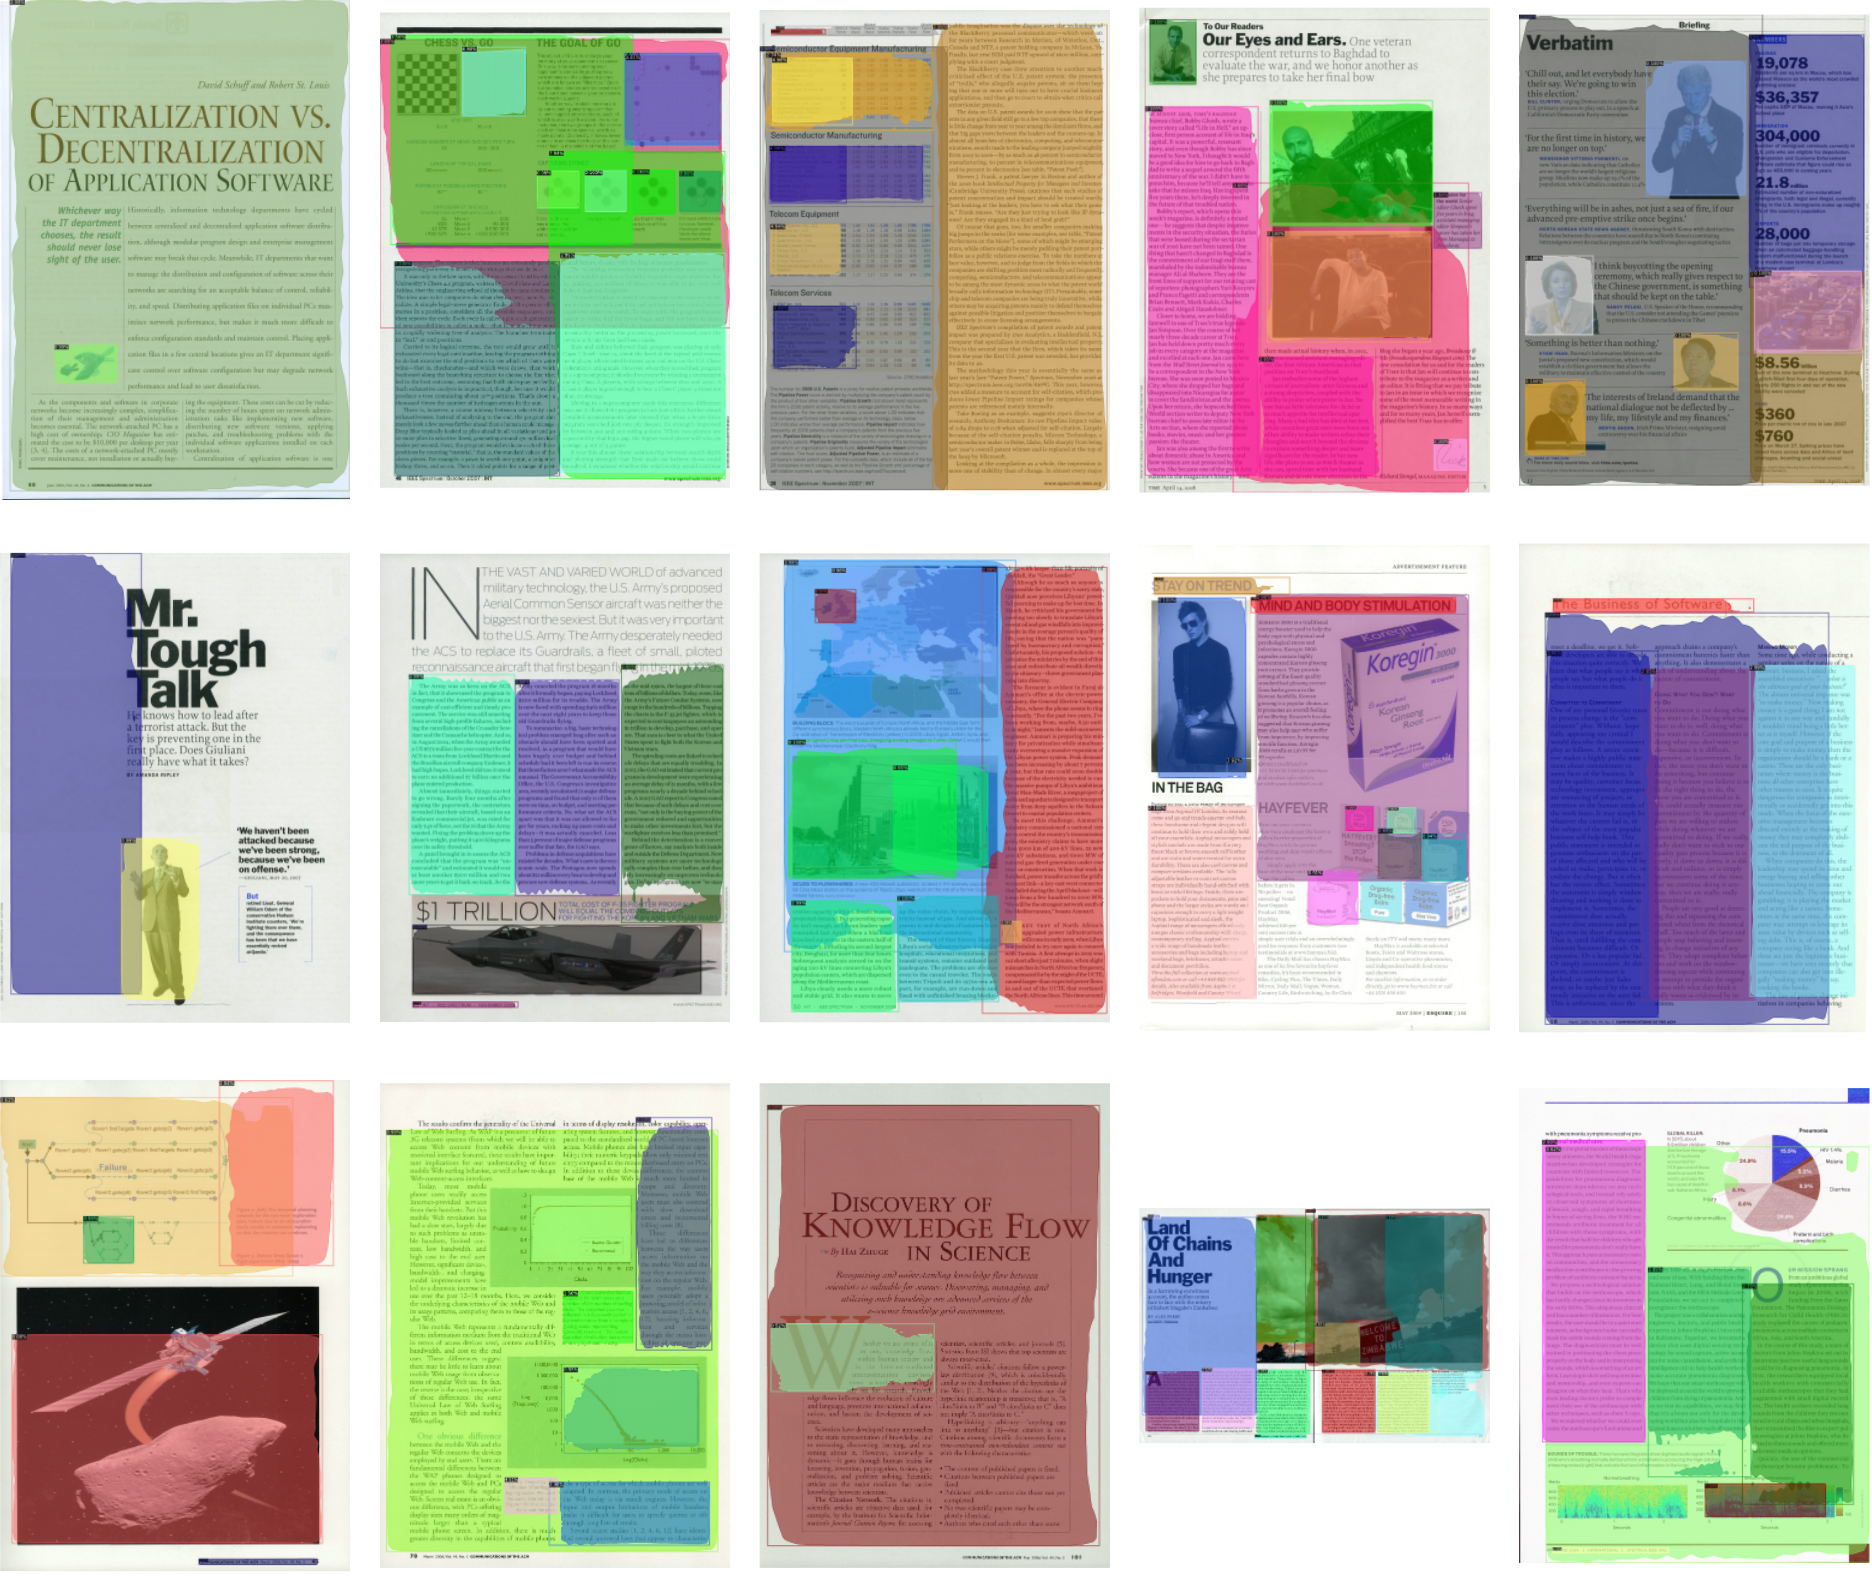
\includegraphics[width=\linewidth]{LaTeX/Figures/RDCL-2019.png}
%   \caption{Example of Mask R-CNN Results on RDCL-2019 Dataset}
%   \label{fig:rdcl19}
%  \end{figure}


%  \begin{figure}[]
%   \centering
%   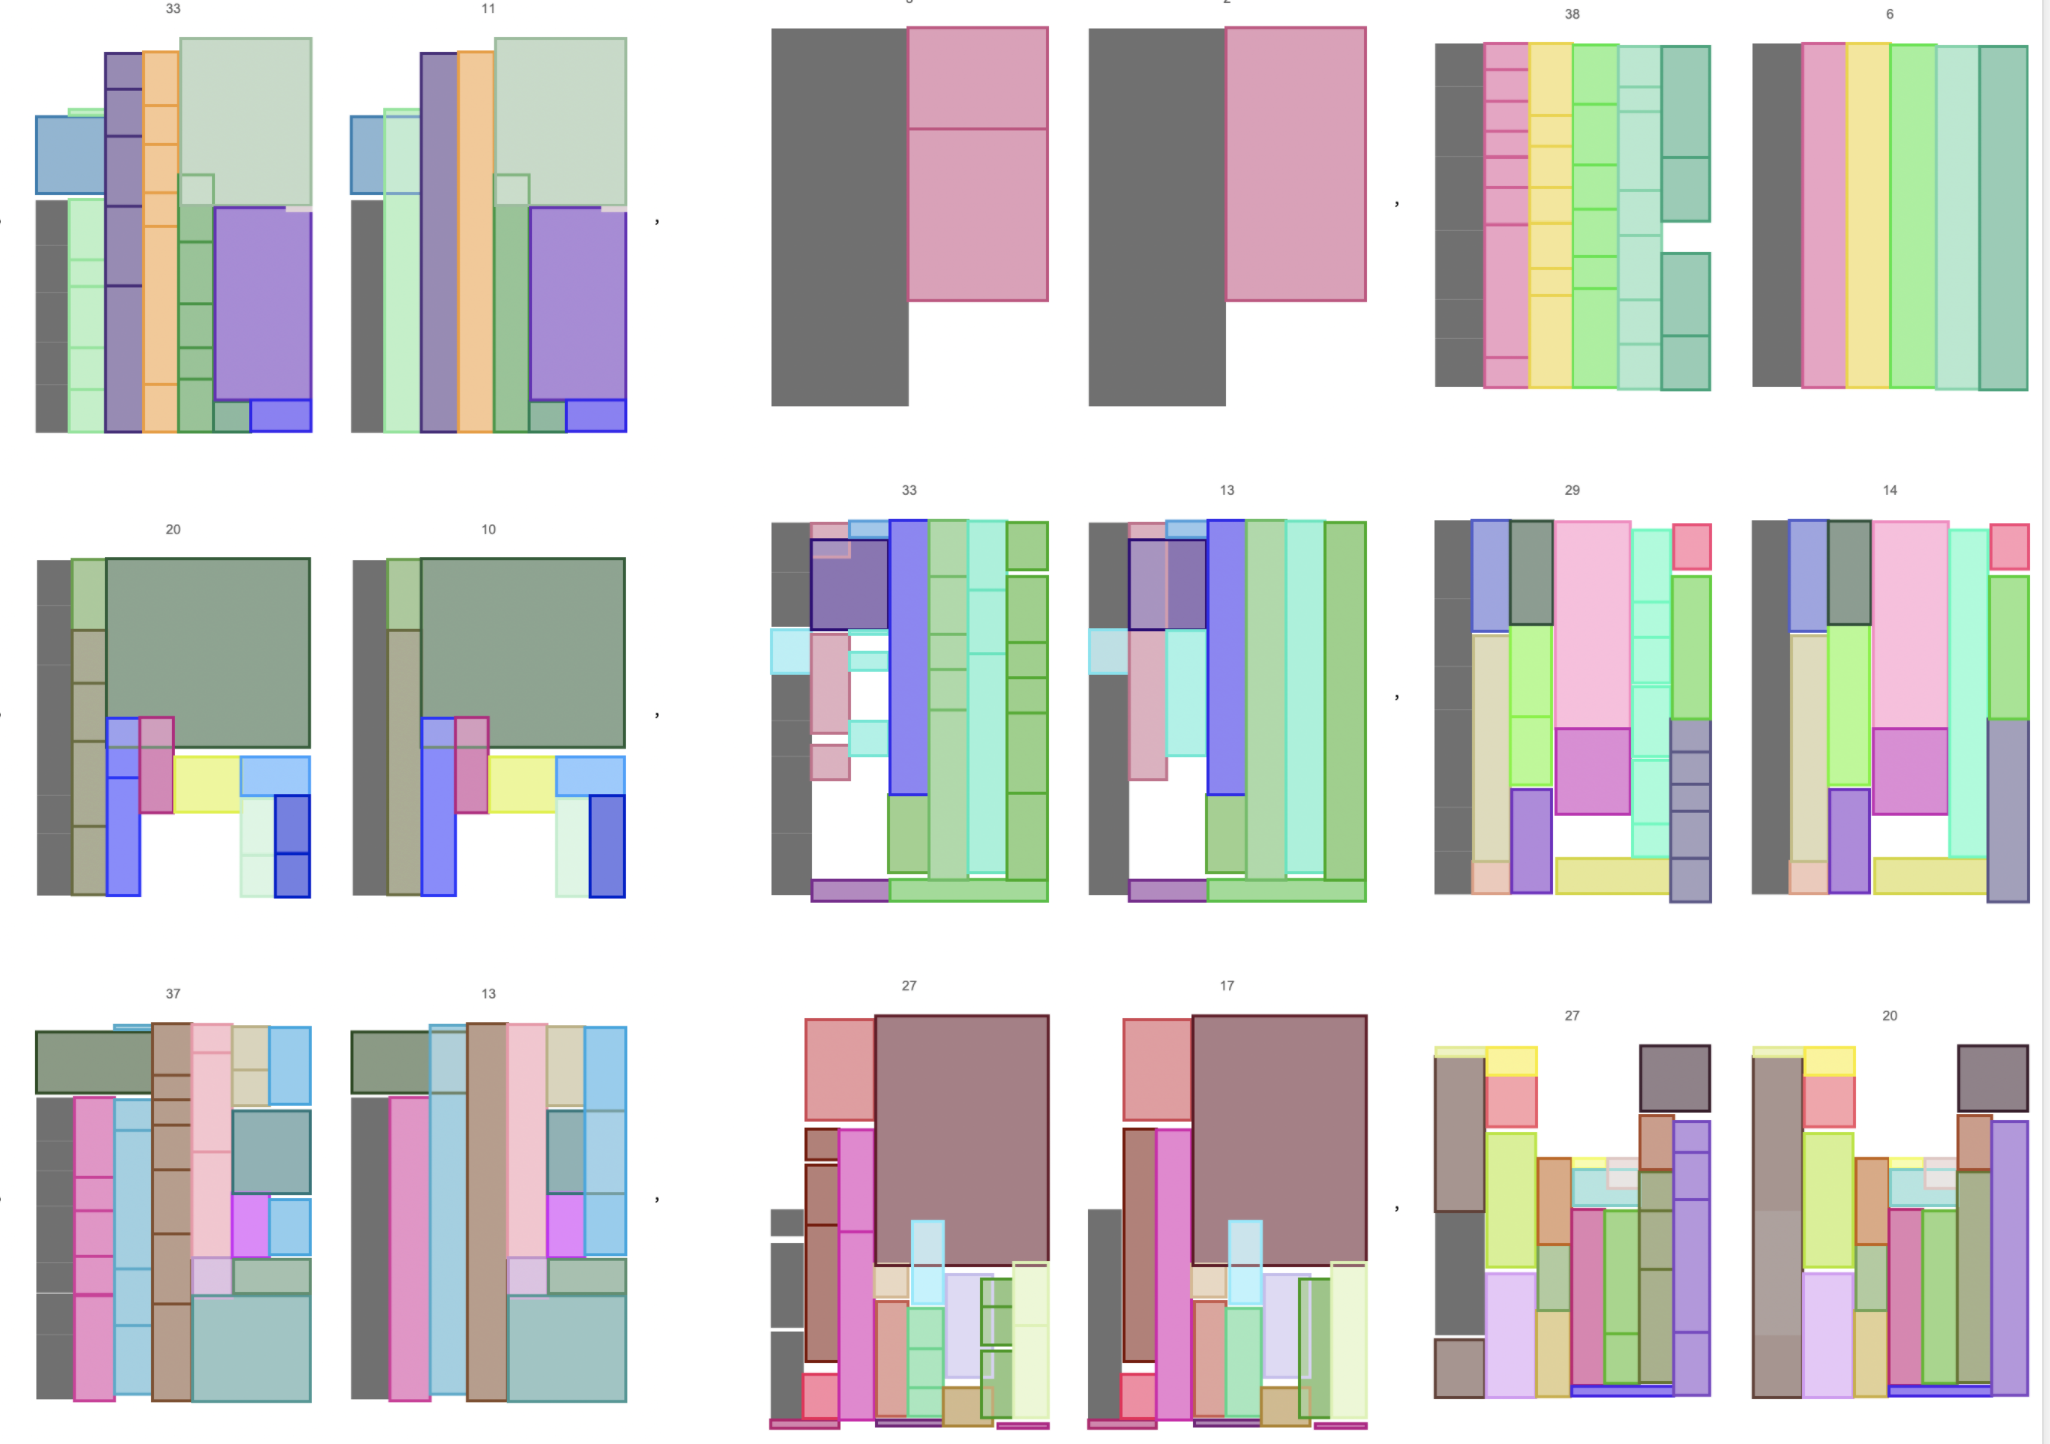
\includegraphics[width=\linewidth]{LaTeX/Figures/bbox_post.png}
%   \caption{Visualization of geometric post-processing step applied on the layout}
%   \label{fig:pp}
%  \end{figure}
 
 \bigskip
\end{document}